%%%%%%%% ICML 2025 EXAMPLE LATEX SUBMISSION FILE %%%%%%%%%%%%%%%%%

\documentclass{article}

% Recommended, but optional, packages for figures and better typesetting:
\usepackage{microtype}
\usepackage{graphicx}
\usepackage{subfigure}
\usepackage{booktabs} % for professional tables
\usepackage{tcolorbox}
\usepackage{tabularx}
\usepackage{rotating}
\usepackage{placeins}
\usepackage{cancel}
\usepackage{physics}
\usepackage[hyphens]{url}


% hyperref makes hyperlinks in the resulting PDF.
% If your build breaks (sometimes temporarily if a hyperlink spans a page)
% please comment out the following usepackage line and replace
% \usepackage{icml2025} with \usepackage[nohyperref]{icml2025} above.
\usepackage{hyperref}
\newcommand\johan[1]{\noindent{\color{orange} {\bf \fbox{Johan}} {\it#1}}}

\newcommand\hugh[1]{\noindent{\color{green} {\bf \fbox{Hugh}} {\it#1}}}

% Attempt to make hyperref and algorithmic work together better:
\newcommand{\theHalgorithm}{\arabic{algorithm}}

% Use the following line for the initial blind version submitted for review:
\usepackage[accepted]{icml2025}

% If accepted, instead use the following line for the camera-ready submission:
%\usepackage[accepted]{icml2025}

% For theorems and such
\usepackage{amsmath}
\usepackage{amssymb}
\usepackage{mathtools}
\usepackage{amsthm}

% if you use cleveref..
\usepackage[capitalize,noabbrev]{cleveref}

\input{math_commands.tex}

%%%%%%%%%%%%%%%%%%%%%%%%%%%%%%%%
% THEOREMS
%%%%%%%%%%%%%%%%%%%%%%%%%%%%%%%%
\theoremstyle{plain}
\newtheorem{theorem}{Theorem}[section]
\newtheorem{proposition}[theorem]{Proposition}
\newtheorem{lemma}[theorem]{Lemma}
\newtheorem{corollary}[theorem]{Corollary}
\theoremstyle{definition}
\newtheorem{definition}[theorem]{Definition}
\newtheorem{assumption}[theorem]{Assumption}
\theoremstyle{remark}
\newtheorem{remark}[theorem]{Remark}
\usepackage{etoc}

% Todonotes is useful during development; simply uncomment the next line
%    and comment out the line below the next line to turn off comments
%\usepackage[disable,textsize=tiny]{todonotes}
\usepackage[textsize=tiny]{todonotes}
% 1. Equation: "Eq." and "Eqs."
\Crefname{equation}{Eq.}{Eqs.}
\crefname{equation}{Eq.}{Eqs.}

% 2. Figure: "Fig." and "Figs."
\Crefname{figure}{Fig.}{Figs.}
\crefname{figure}{Fig.}{Figs.}

% 3. Section: "Sec." and "Secs."
\Crefname{section}{Sec.}{Secs.}
\crefname{section}{Sec.}{Secs.}

% Appendix: "App." and "Apps."
\Crefname{appendix}{App.}{Apps.}
\crefname{appendix}{App.}{Apps.}

\definecolor{darkmagenta}{rgb}{0.56, 0.0, 1.0} 
\usepackage{multirow}
\usepackage{inconsolata}
\usepackage{changepage} % in preamble
\usepackage{newtxmath}
\hypersetup{colorlinks,linkcolor={orange},citecolor={darkmagenta},urlcolor={orange}} 
\hypersetup{colorlinks,linkcolor={blue},citecolor={darkmagenta},urlcolor={blue}} 

% The \icmltitle you define below is probably too long as a header.
% Therefore, a short form for the running title is supplied here:
\icmltitlerunning{A Mechanistic Analysis of Looped Language Models}

\makeatletter
\def\addcontentsline#1#2#3{%
\addtocontents{#1}{\protect\contentsline{#2}{#3}{\thepage}{\@currentHref}{}}}
\makeatother
\begin{document}
\etocdepthtag.toc{mtoc}
\etocsettagdepth{mtoc}{none}
\etocsettagdepth{appendix}{none}

% 2. Generate the invisible TOC (Only the print command goes in the box)
\newbox\dummybox
\setbox\dummybox\vbox{%
  \tableofcontents 
}

% MPL colors for describing the colormaps
\definecolor{mplwinterblue}{RGB}{0, 0, 219}
\definecolor{mplwintergreen}{RGB}{0, 219, 96}
\definecolor{mplsummergreen}{RGB}{0, 96, 72}
\definecolor{mplsummeryellow}{RGB}{219, 219, 91}


\twocolumn[
\icmltitle{A Mechanistic Analysis of Looped Reasoning Language Models}

% It is OKAY to include author information, even for blind
% submissions: the style file will automatically remove it for you
% unless you've provided the [accepted] option to the icml2025
% package.

% List of affiliations: The first argument should be a (short)
% identifier you will use later to specify author affiliations
% Academic affiliations should list Department, University, City, Region, Country
% Industry affiliations should list Company, City, Region, Country

% You can specify symbols, otherwise they are numbered in order.
% Ideally, you should not use this facility. Affiliations will be numbered
% in order of appearance and this is the preferred way.
\icmlsetsymbol{equal}{*}

\begin{icmlauthorlist}
\icmlauthor{Hugh Blayney}{Ox}
\icmlauthor{Álvaro Arroyo}{Ox}
\icmlauthor{Johan Obando-Ceron}{Mila,Mont}
\\
\icmlauthor{Pablo Samuel Castro}{Mila,Mont} 
\icmlauthor{Aaron Courville}{Mila,Mont}
\icmlauthor{Michael Bronstein}{Ox,AITHYRA}
\icmlauthor{Xiaowen Dong}{Ox}
%\icmlauthor{}{sch}
%\icmlauthor{}{sch}
%\icmlauthor{}{sch}
\end{icmlauthorlist}

\icmlaffiliation{Ox}{University of Oxford}
\icmlaffiliation{Mila}{Mila – Quebec AI Institute}
\icmlaffiliation{Mont}{Universit\'e de Montr\'eal}
% \icmlaffiliation{GDM}{School of ZZZ, Institute of WWW, Location, Country}
\icmlaffiliation{AITHYRA}{AITHYRA}
\icmlcorrespondingauthor{Hugh Blayney}{hugh@robots.ox.ac.uk}
\icmlcorrespondingauthor{Álvaro Arroyo}{alvaro.arroyo@eng.ox.ac.uk}

% You may provide any keywords that you
% find helpful for describing your paper; these are used to populate
% the "keywords" metadata in the PDF but will not be shown in the document
\icmlkeywords{Machine Learning, ICML}

\vskip 0.3in
]

% this must go after the closing bracket ] following \twocolumn[ ...

% This command actually creates the footnote in the first column
% listing the affiliations and the copyright notice.
% The command takes one argument, which is text to display at the start of the footnote.
% The \icmlEqualContribution command is standard text for equal contribution.
% Remove it (just {}) if you do not need this facility.

\printArXivAffiliationsAndNotice{}
%\printAffiliationsAndNotice{}  % leave blank if no need to mention equal contribution
%\printAffiliationsAndNotice{\icmlEqualContribution} % otherwise use the standard text.

\begin{abstract}
    Reasoning has become a central capability in large language models. Recent research has shown that reasoning performance can be improved by looping an LLM’s layers in the latent dimension, resulting in \textit{looped reasoning language models}. Despite promising results, few works have investigated how their internal dynamics differ from those of standard feedforward models. In this paper, we conduct a mechanistic analysis of the latent states in looped language models, focusing in particular on how the \textit{stages of inference} observed in feedforward models compare to those observed in looped ones. To this end, we analyze cyclic recurrence and show that for many of the studied models each layer in the cycle converges to a distinct fixed point; consequently, the recurrent block follows a consistent cyclic trajectory in the latent space. We provide evidence that as these fixed points are reached, attention-head behavior stabilizes, leading to constant behavior across recurrences. Empirically, we discover that recurrent blocks learn stages of inference that closely mirror those of feedforward models, repeating these stages in depth with each iteration. We study how recurrent block size, input injection, and normalization influence the emergence and stability of these cyclic fixed points. We believe these findings help translate mechanistic insights into practical guidance for architectural design.    
\end{abstract}

\section{Introduction}\label{sec:intro}
The vast majority of current LLMs are based on the Transformer architecture \cite{vaswani2017attention}, which comprises a sequence of blocks traversed in a feedforward manner to predict the next token. As the capability of these models increased, attention turned to eliciting \textit{reasoning} capabilities in LLMs by increasing test-time computation, commonly through chain-of-thought (CoT) prompting \cite{wei2022chain} or reinforcement-learning-based fine-tuning, first popularized in the DeepSeek-R1 architecture \cite{guo2025deepseek}. More recently, research has explored building reasoning capabilities directly into the model architecture via \textit{recurrent looping} \cite{geiping2025scaling, wang2025hierarchical, jolicoeur2025less}, where additional test-time compute is spent by taking more recurrent steps, echoing early designs in this direction \cite{graves2016adaptive}. Despite growing empirical success, the mechanisms underlying these models remain poorly understood, as well as their benefits and limitations when compared to feedforward computation.


\begin{figure}[!t]
    \centering
    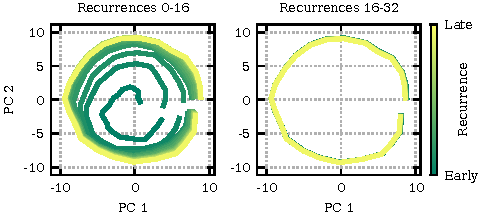
\includegraphics[width=\linewidth]{figures/splash_trajectory.pdf}
    \vspace{-0.91cm}
    \caption{\textbf{Latent states after each block in a recurrent model frequently tend towards \emph{separate} fixed points}, meaning that the application of a recurrent block tends towards a consistent trajectory in latent space.}
    \vspace{-0.5cm}
    \label{fig:random_trajectory}
\end{figure}

In this paper, we compare how feedforward and looped LLMs organize computation across (effective) depth through the lens of \textit{stages of inference} \citep{lad2024remarkable, queipo2025attention}, a perspective suggesting that LLM inference can be decomposed into several distinct computational stages. Building on prior observations that repeated application of a shared recurrent block can approach a fixed point or steady state \citep{yang2023looped, geiping2025scaling}, we show that such behavior necessarily implies one of two possibilities: either the contribution of the component Transformer blocks vanishes asymptotically, or their sequential application traces out a \textit{constant cyclic trajectory} in latent space. We further demonstrate empirically that the latter behavior arises in practice when certain architectural conditions are met, and that this appears to be emergent behavior from the Transformer architecture itself, appearing in both trained recurrent models and untrained, randomly initialized models.

\begin{tcolorbox}[colback=orange!10,
leftrule=0.5mm,top=1mm,bottom=1mm,boxrule=0.6pt]
\paragraph{Our analysis yields two key insights:}
\begin{enumerate}
    \item \Cref{sec:cyclic_similarity} establishes that many looped language models tend toward \emph{cyclic fixed-point} behavior, providing theoretical and empirical proof that this implies convergence to fixed attention patterns. \Cref{subsec:norm_and_ii} explores how specific architectural choices influence this behavior.
    \item \Cref{sec:stages_of_inference} demonstrates that these stable attention patterns mirror the ``mixing'' stages of inference learned in feedforward models. We then provide evidence in \Cref{sec:self_organising_soi} that models naturally self-organize into these stages during training, and show in \Cref{sec:stability} that stable fixed-point models successfully maintain these inference stages, whereas unstable models deviate.
\end{enumerate}
\end{tcolorbox}






\section{Preliminaries}\label{sec:prelim}
\subsection{Looped Transformers}

In this section we introduce Looped Transformers and define the notation that we will use throughout the paper. We represent the input sequence to our transformer of length $T$ and dimension $D$ as $\mX \in \mathbb{R}^{T \times D}$. Following the notation of \citet{yudin2025pay} we define $\attn$, the dot product self-attention mechanism, as a map $f: \mathbb{R}^{T \times D} \to \mathbb{R}^{T \times D}$:
\begin{align}
    \attn(\mX) &= \softmax{\left ( \frac{\mX \mW_Q \mW_K^{\top} \mX^{\top}}{\sqrt{d}} \right )} \mX\mW_V, \\ 
    &= \softmax{\left ( A(\mX) \right )} \mX\mW_V, \label{eq:attn_in_a}
\end{align}
where $\mW_Q, \mW_K, \mW_V \in \mathbb{R}^{D \times d}$ are projection matrices and $A$ is defined for convenience. 

A transformer block typically comprises an attention mechanism and a position-wise MLP as follows:
\begin{align}
    \hat{\mX} &= n_2 \left ( \mX + \attn(n_1(\mX) \right ), \label{eq:block_norm_1} \\
    {\mX}' &= n_4 \left ( \hat{\mX} + \text{MLP}(n_3(\hat{\mX})) \right ), \label{eq:block_norm_2}
\end{align}
where $n_1, n_2, n_3, n_4$ are each optional norms -- here we are borrowing from the notation of \citet{geiping2025scaling}. We denote the action of a Transformer block $\block: \mathbb{R}^{T \times D} \to \mathbb{R}^{T \times D}$ as $\mX' = \block(\mX)$, and refer to the intermediate hidden-state matrices $\mX$ between blocks as the \textbf{residual stream}.
% We will denote the action of this Transformer block $\block: \mathbb{R}^{T \times D} \to \mathbb{R}^{T \times D}$ as
% \begin{equation}
%     {\mX}' = \block(\mX),
% \end{equation}

% and the matrices $\mX$ of hidden states between Transformer blocks we will frequently refer to as the \textbf{residual stream}.

Looped Transformers are Transformers that utilize ``recurrence in depth'' -- that is, they reapply layers to repeatedly act on the latent states. Recent research has identified that an effective way \citep{bae2025mixture} to achieve this is via \emph{cyclic recurrence}: a fixed sequence of layers is repeated in a ``cyclic'' pattern. This is the approach that we focus on in this work, and we introduce it in more detail below. For convenience, we define a $k$-stacked block as a composition of Transformer blocks,
$\stack_k(\mX) = \block_k(\block_{k-1}(\dots \block_1(\mX) \dots))$.


% For convenience, we define a $k$-stacked block  comprising a sequence of separate Transformer blocks:
% \begin{equation}
%     \stack_k(\mX) = \block_k(\block_{k-1}( \dots \block_1(\mX) \dots ))
% \end{equation}

In the case of \citet{geiping2025scaling,mcleish2025teaching} this stacked block may also take an additional input $\mZ \in \mathbb{R}^{T \times D}$ which is typically initialized from a Normal distribution, as well as the original input to the recurrent section: this is known as \emph{input injection} \citep{bai2019deep,anil2022path}, and the two inputs are projected into common feature space $\mathbb{R}^D$ before the block is applied. In the case of input injection, a $k$-stacked block therefore becomes
\begin{equation}
    \stack_k(\mX, \mZ) = \block_k ( \block_{k-1}( \dots \block_1([\mX, \mZ] \mW_I) \dots )),
\end{equation}
where $[\cdot, \cdot]$ denotes concatenation in the channel dimension and $\mW_I \in \mathbb{R}^{2D \times D}$ is a learned projection matrix.

This allows us to define a $(k \otimes l)$-Recurrent block as a $k$-stacked block repeated $l$ times:
\begin{equation}
    R_{l,k}(\mX) = \overbrace{\stack_k ( \stack_{k}( \dots \stack_k(}^{\times l} \mX) \dots )),
\end{equation}

which with input-injection becomes
\begin{equation}
    R_{l,k}(\mX, \mZ) = \overbrace{\stack_k ( \mX, \stack_{k}( \dots \mX, \stack_k( \mX, \mZ)) \dots ))}^{\times l}.
\end{equation}

Note that the input $\mX$ is only ``injected'' at the start of each stack of blocks -- once per recurrence. Additionally, a complete looped Transformer may have multiple feedforward layers before the Recurrent block, and multiple feedforward layers after the Recurrent block: following the convention of \citet{geiping2025scaling}, we refer to these as \emph{prelude} and \emph{coda} layers respectively, and these are simply separate stacked blocks with non-tied layer weights. Where prelude and coda are used, we will frequently refer to this as a \emph{sandwich} block structure.

We combine and adapt the nomenclature of \citet{geiping2025scaling,saunshi2025reasoning} and refer to a looped Transformer with $p$ prelude layers, $k$ recurrent layers and $c$ coda layers with the tuple $(p, k, c)$. Where input injection is used, we add an $I$ subscript $(p, k, c)_I$, and when referring to a recurrent layer looped a specific number of times $l$, we denote this as $(p, k \otimes l, c)$.

In summary, a $(p, k \otimes l, c)$ looped Transformer is defined as
\begin{align*}
    \mX_0 &\gets \stack_p(\mX) \\
    \mX_i &\gets \stack_{k}^{\prime}(\mX_{i-1}) \qquad i \in \{1, \dots, l \} \\
    \mX &\gets \stack_c^{\prime \prime}(\mX_l),
\end{align*}
where $\prime$ and $\prime \prime$ indicates that these are \emph{different} stacks between which weights are not shared. A $(p, k \otimes l, c)_I$ looped Transformer (with input injection) is defined as
\begin{align*}
    \mX &\gets \stack_p(\mX) \\
    \mZ_i &\gets \stack_{k}^{\prime}(\mX, \mZ_{i-1}) \qquad i \in \{1, \dots, l \} \\
    \mX &\gets \stack_c^{\prime \prime}(\mZ_l),
\end{align*}
where $\mZ_0$ is initialized such that each column is sampled from $\mathcal{N}(\boldsymbol{0}, \sigma^2 \mathbb{I}_{D})$.

% We will often refer to the depth of the entire looped model -- summing the depth of stacked layers -- as the \textbf{realized depth}, and the depth of the cyclic recurrent block as the \textbf{recurrent depth}.

We will describe our results via \textbf{grouping}:
\begin{itemize}
    \item \textbf{No grouping}: The value is visualized as it evolves through sequential layers of the model, irrespective of whether these layers are repeated.
    \item \textbf{By recurrence}: Separate lines are visualized for each complete pass through the recurrent block. The $x$-axis is typically percentage scaled to represent relative depth within that block (including prelude/coda), allowing us to overlay and compare successive passes. Always presented with a \textbf{\textcolor{mplsummergreen}{green}-\textcolor{mplsummeryellow}{yellow}} colorbar, with later recurrences colored more yellow.
    \item \textbf{By layer}: Separate lines are visualized for each unique layer, showing how the value evolves across recurrences. Always presented with a \textbf{\textcolor{mplwinterblue}{blue}-\textcolor{mplwintergreen}{green}} colorbar, with later layers colored more green.
\end{itemize}

\subsection{Stages of Inference}\label{subsec:stages_of_inference_prelim}

The behavior of layers in feedforward Transformers appears to change sharply with depth: \citet{lad2024remarkable} originate the term ``stages of inference'' and demonstrate how several different layer mechanisms emerge at different depths. \citet{queipo2025attention} further develop this viewpoint, focusing on behaviors that can be characterized by the \emph{mixing} (or lack thereof) induced by the attention heads. We focus on this latter perspective.
% For a representation matrix $\mathbf{X}$ with singular values $\sigma_1 \geq \sigma_2 \geq \ldots \geq \sigma_r$, we measure compression via the \textbf{matrix-based entropy}:
% \begin{equation}
% H(\mathbf{X}) = -\sum_{j=1}^r p_j \log p_j, \\ \text{where } p_j = \sigma_j^2/\|\mathbf{X}\|_F^2
% \end{equation}
% Low entropy indicates compression into few dominant directions. The \textbf{anisotropy} $p_1 = \sigma_1^2/\|\mathbf{X}\|_F^2$ measures directional bias~\citep{razzhigaev2024shapelearninganisotropyintrinsic} (near 1 = extreme bias, near $1/r$ = isotropy).
Mixing in this context refers to the extent to which the attention mechanism incorporates information from previous tokens at each layer. Throughout the main text of this paper we quantify our study of mixing behavior through the \emph{ColSum Concentration} metric introduced in \citet{queipo2025attention}; we introduce and discuss additional metrics in \Cref{appen:additional_soi_results}.

We first define the column sum $c_j = \sum_i A_{ij}$ to capture how much attention mass is received by token $j$. We normalize this as $\hat{c}_j = c_j / T$ to obtain a probability distribution, noting that $\sum_{i,j} A_{ij} = T$ since $A$ is row-stochastic. From this distribution, we define the \textbf{ColSum Concentration} via its normalized entropy as
$C = 1 - H_{\text{col}} \in [0,1] = 1 + \frac{1}{\log T} \sum_j c_j \log c_j$.
 

% From this distribution we define the \textbf{ColSum Concentration} from its normalized entropy:
% \begin{align}
%     C &= 1 - H_{\text{col}} \in [0,1] \\
%     &= 1 + \frac{1}{\log{T}} \sum_j c_j \log{c_j}
% \end{align}
Large values of $C$ indicate a high \emph{concentration} of attention mass: few columns receive most of the mass. We note therefore that this metric captures the well-studied \emph{attention sink} \citep{xiao2023efficient,barbero2025llms} behavior, but generalizes to capture concentration over any token position. This property is useful for our investigation as not all models studied herein exhibit sinks on the first token; in particular OLMo-2 frequently concentrates attention mass on punctuation, echoing a result in \citet{sandoval2025using}.

\section{Related Work}\label{sec:related_work}
% \textcolor{red}{Here, we ....}
\paragraph{Looped and Recurrent Transformers}

Reusing the same Transformer block for multiple iterations is an idea that has been explored in the literature. This began with the introduction of Universal Transformers  \cite{dehghani2018universal}, which have also resulted in sparsified and conditional-computation extensions \cite{tan2023sparse,csordas2024moeut}. Other more recent recurrent style architectures with a higher focus on reasoning-style tasks have been HRM \cite{wang2025hierarchical} and TRM \cite{jolicoeur2025less}. Within language modeling, we highlight \raven{} \cite{geiping2025scaling}, \ouro{} \cite{zhu2025scaling}, and Mixture-of-Recursions \citep{bae2025mixture} as models that have been pretrained from random initialization, as well as recent work by \citep{mcleish2025teaching, koishekenov2025encode} that retrofit recurrence into pretrained LLMs.  

In terms of mechanistic studies, we highlight \citet{pappone2025two}, who analyze “two-scale” latent dynamics in recurrent Transformers. However, the setting of their analysis is different from ours: they analyse a model in which each recurrent block comprises either 1 or 2 layers, and the model comprises multiple \emph{separate} recurrent blocks. In this way, the two scales they refer to correspond to the outputs of each iteration of a given recurrent block, and outputs of recurrent blocks when transitioning between different recurrent blocks. We instead study a single looped block with deeper cycles (4+ layers), closer to common looped architectures, and we analyze the internals of these cyclic blocks by examining the latent states of each separate layer. We also highlight work related to looped model expressivity \citep{xu2024expressive, saunshi2025reasoning}, as well as work on neural network stability and fixed-point dynamics \citep{bai2019deep, anil2022path, ke2024advancing, yudin2025pay}. The only work -- of which we are aware -- that analyses the internal states of the cyclic recurrent blocks is \citet{lu2025latent}, who demonstrate cyclic behavior in logit lens prediction throughout recurrent blocks.



\paragraph{Stages of Inference and Attention Dynamics}

The idea that LLMs organize their feedforward computation into several distinct \textit{stages of inference} was first proposed by \citet{lad2024remarkable}. Building on this, \citet{queipo2025attention} explain the emergence of these stages through the behavior of attention heads, driven by massive activations \citep{sun2024massive}. We also highlight a complementary line of work that analyzes LLM learning dynamics via attention patterns through the lens of \textit{mixing} \citep{barbero2024transformers, arroyo2026a, velivckovic2024softmax, barbero2025llms}, motivated by information propagation challenges originally studied in Graph Neural Networks (GNNs) \citep{cai2020note,alon2020bottleneck,arroyo2025vanishing,hariri2025return,blayney2025glstm}.

\paragraph{Test-time Computation}

Test-time computation broadly refers to giving a model the ability to expend additional computational cycles at inference in proportion to the difficulty of the input, rather than committing to a fixed compute budget for all examples. In this paper, we focus specifically on \emph{recurrence} as a mechanism for scaling computation at test time, as opposed to alternative strategies such as early-exit architectures \cite{schuster2022confident} or continuous thought machines \cite{darlow2025continuous}. Classic approaches to adaptive test-time compute include Adaptive Computation Time \cite{graves2016adaptive} and subsequent probabilistic halting frameworks such as PonderNet \cite{banino2021pondernet}. Building on these foundations, recent work has begun to characterize when additional inference compute actually generalizes beyond training-time budgets \cite{schwarzschild2021can}, how to mitigate failures due to excessive computation (``overthinking'') \citep{bansal2022end}, how to ensure stable dynamics with repeated iteration \citep{bear2024rethinking}, and how looped Transformers can better generalize to out of distribution tasks at test time \citep{mcleish2024transformers}.










\begin{figure*}[ht]
    \centering
    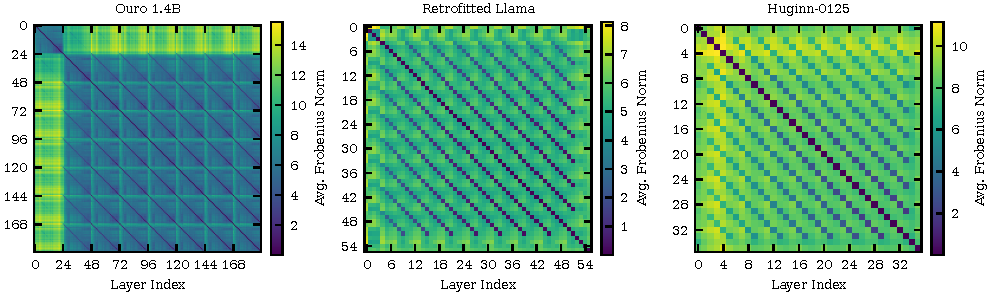
\includegraphics[width=0.8\linewidth]{figures/fixed_point/heatmaps/attention_weight_norms.pdf}
    \vspace{-0.3cm}
    \caption{\textbf{Frobenius norm between attention patterns at different depths}, averaged across the batch and head dimensions. Depth index visualized on each axis, cells show the norms between attention patterns at each pair of depth indices. \textbf{Left:} Ouro 1.4B \citep{zhu2025scaling}. \textbf{Center:} Retrofitted Llama \citep{mcleish2025teaching}. \textbf{Right:} \raven{} \citep{geiping2025scaling}. All models looped 8 times.}
    \vspace{-0.3cm}
    \label{fig:similar_attention_patterns}
\end{figure*}

% \section{The tendency towards attention homogeneity in looped models}
\section{Looped Transformers Tend Towards the Same Attention Patterns}\label{sec:cyclic_similarity}

Recent work \citep{bai2019deep,bansal2022end,anil2022path} has noted that weight-tied Transformer models often tend towards consistent behavior with repeated iterations. Often\footnote{As originally observed by \citet{geiping2025scaling}, other forms of limiting behavior can occur. In \Cref{appen:orbits_and_sliders} we show that 1) this is rare, the vast majority of tokens reach a fixed-point and 2) even with other limiting behavior, stages of inference remain constant.}, this takes the form of convergence to a fixed point $\mX' = \stack_k(\mX')$. We motivate our work by noting that if this is true for a model with cyclic recurrence, it is also true cyclically:

\begin{proposition}[Cyclic recurrent blocks reach cyclic fixed points]\label{prop:cyclic_fixed_point}
    Let $(l, k)$-Recurrent block reach a fixed point $\mX'$ such that $\stack_k(\mX') = \mX'$. Then any cyclic permutation of blocks $1, \dots, k$ will also have reached a fixed point.
\end{proposition}

We highlight however that these fixed points are not necessarily the same: the action of each successive layer doesn't necessarily result in the same point, and the cycle of layers can instead trace out an arbitrary cycle in latent space. Indeed, in \Cref{subsec:fixed_point_empirical} we demonstrate that this \emph{cyclic fixed point} behavior -- illustrated in \Cref{fig:random_trajectory} -- is observed frequently in practice. The alternative, where all layers result in the same fixed point, requires that the action of each Transformer block tends to zero.

% We additionally note that this is true \emph{cyclically} - for cyclically looped transformers, every sub-cycle tends towards a separate fixed point: see \Cref{fig:untrained_fixed_point} for evidence of this in an untrained transformer block and \Cref{fig:pretrained_pythia_fixed_point} for evidence of this when stacking pretrained Pythia.

Convergence to this cyclic behavior implies that the residual stream tends towards being similar across recurrences. Given that block weights are also shared across recurrent iterations -- and assuming that the inputs to each block are bounded\footnote{This is a reasonable assumption since all models considered in this work apply a norm before the attention block.} -- this implies that the attention patterns will converge, as shown in \Cref{prop:similar_attention_patterns}.

\begin{proposition}[Recurrent attention patterns change slowly under state convergence]\label{prop:similar_attention_patterns}
Fix a layer $\ell$ in the recurrent block and consider its attention weight matrices to be tied across recurrences (so $\mW_{Q,\ell},\mW_{K,\ell}$ are the same for all $t$). 
Let $\|\cdot\|$ denote a submultiplicative matrix norm that is invariant under transposition (e.g. Spectral or Frobenius norms). Assume the corresponding attention inputs are bounded under this norm as $\|\mX_{\ell,t}\|\le B$ for all $t$. Define $\kappa_\ell = \|\mW_{Q,\ell}\mW_{K,\ell}^\top\|$.  
Then, writing $\mathcal S_\ell(\mX):=\softmax(A_\ell(\mX))$ with $A_\ell(\cdot)$ as defined above, for any $t\ge 1$,
\begin{equation*}\label{eq:recurrent_attention_lip}
\big\|\mathcal S_\ell(\mX_{\ell,t})-\mathcal S_\ell(\mX_{\ell,t-1})\big\|
\;\le\;
L_{\mathrm{sm}}\,
\frac{2B\,\kappa_\ell}{\sqrt d}\,
\big\|\mX_{\ell,t}-\mX_{\ell,t-1}\big\|,
\end{equation*}
where $L_{\mathrm{sm}}$ is a Lipschitz constant of the row-wise softmax with respect to the chosen norm. 
\end{proposition}

Since these attention patterns are characteristic of the different mixing stages of inference (defining, for example, ColSum concentration), we see that mixing behavior will tend towards being constant across recurrences.



\subsection{Empirical Validation}\label{subsec:fixed_point_empirical}

We focus our attention on three different pretrained looped language models: \ouro{} 1.4B \citep{zhu2025scaling}, \raven{} \citep{geiping2025scaling}, and Llama with retrofitted recurrence \citep{mcleish2025teaching}. Additional models can be found in \Cref{appen:additional_fixed_point_results}, with architecture and training choices summarized in \Cref{tab:looped_model_details}. These models cover a range of design choices; later in \Cref{subsec:norm_and_ii} we will isolate the impact of these architectural differences. Except where otherwise specified, all results are visualized on the same random subset of 256 examples from the GSM8k test set; additional results targetting non-reasoning behavior are presented in \Cref{appen:hellaswag_soi}, but we observe no significant changes and the conclusions of the main text remain unchanged.

\begin{figure}[ht]
    \centering
    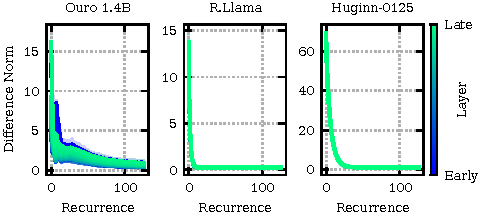
\includegraphics{figures/fixed_point/recurrencewise/successive_difference_norms.pdf}
    \vspace{-0.4cm}
    \caption{\textbf{Norm of the difference between the residual stream after successive recurrences of the same layer.}}
    \vspace{-0.4cm}
    \label{fig:successive_norms}
\end{figure}

We start by plotting the norm of the residual stream difference between subsequent iterations in \Cref{fig:successive_norms} (and the same for cosine similarities in \Cref{fig:successive_cosine_similarities}). This validates the starting assumption of \Cref{prop:similar_attention_patterns} that looped models tend towards behavior in which the layerwise residual stream does not significantly change between recurrences.

For each of these models, we plot Frobenius norm between the realized attention matrices at different layers, for 8 loops of the recurrent block in \Cref{fig:similar_attention_patterns}. The diagonal patterns of high similarity demonstrate that the attention matrices of any given layer are most similar to those of the same layer at different recurrences -- as predicted by \Cref{prop:similar_attention_patterns}. We note that this convergence towards similar attention patterns occurs \emph{remarkably quickly}: for looped \ouro{} attention patterns appear to converge after the first iteration, and both \raven{} and the retrofitted Llama model demonstrate this cyclic behavior immediately following the prelude.

%layers. Additional results showing similar behavior with residual stream similarity and a wider range of models can be found in \Cref{appen:additional_cyclic_similarity}.

\begin{figure}[ht]
    \centering
    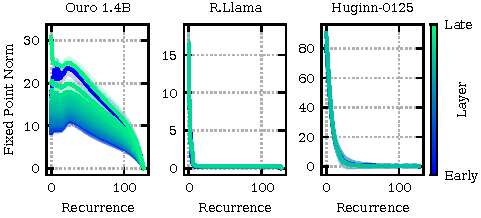
\includegraphics[width=\linewidth]{figures/fixed_point/recurrencewise/fixed_point_norms.pdf}
    \vspace{-0.8cm}
    \caption{\textbf{Norm of the difference between the residual stream after each layer in the recurrent block and its ``approximate fixed point''} - the residual stream after that layer in the 128th recurrence. While \raven{} and retrofitted Llama quickly reach a fixed point, \ouro{} does not - despite small successive differences evidenced by \Cref{fig:successive_norms}.}
    \label{fig:fixed_point_norm}
    \vspace{-0.2cm}
\end{figure}

\begin{figure}[ht]
    \centering
    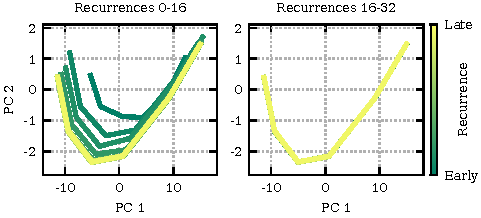
\includegraphics[width=0.9\linewidth]{figures/trajectory/pca_quartiles_Retrofitted_Llama_32_steps.pdf}
    \vspace{-0.5cm}
    \caption{\textbf{Retrofitted Llama \citep{mcleish2025teaching} latent space trajectory traced out by the hidden states of the final sequence position} on a single test prompt; reduced to two dimensions by computing PCA over all final sequence position embeddings. Trajectories perfectly overlap in the second plot, demonstrating that a cyclic fixed point has been reached.}
    \vspace{-0.3cm}
    \label{fig:retro_llama_trajectory}
\end{figure}

However, despite the tendency visible in \Cref{fig:successive_norms} towards small changes between successive iterations we discover that it is \textbf{not} the case that looped models always reach a fixed point, or even consistent limiting behavior: for each model we find an ``approximate fixed point'' per layer by iterating 128 times, then compute the norm of the difference between the output of each layer at every recurrence and its corresponding fixed point. This is visualized in \Cref{fig:fixed_point_norm}. We see that while \raven{} and Retrofitted Llama demonstrate fast convergence to a fixed point, \ouro{} does not. As discussed by \citet{bansal2022end,anil2022path}, this supports the suggestion that input injection encourages fixed-point convergence: we investigate this further in \Cref{subsec:norm_and_ii}.

Where a model does reach a fixed point, this implies that the action of the entire recurrent block tends towards tracing out a consistent cycle in latent space. We visualize this for retrofitted Llama in \Cref{fig:retro_llama_trajectory}.

\subsection{Impact of Architecture Choices}\label{subsec:norm_and_ii}

Several existing works \citep{bansal2022end,anil2022path} have noted that input injection is important in order for a recurrent model to reach a fixed point: in this section we replicate this finding and supplement with additional insights on the impact of norm structure in reaching a fixed point. We conduct a series of experiments on \emph{randomly initialized} models. These demonstrate similar cyclic behavior to their trained counterparts, suggesting that behavior observed here is likely to generalize to the cyclic behavior of trained models. We compare pre-norm (used by the retrofitted recurrent models) and the norms used by the \raven{} and \ouro{} models, testing each both with and without input injection: in this way we test the most significant architectural differences between the pretrained Looped models tested; see \Cref{tab:looped_model_details} for details. Each model has 12 layers with no prelude or coda; see \Cref{fig:stability_initialised_fixed_point_cosine_similarities_multiple_layers} for alternative configurations.

Our results are visualized in \Cref{fig:summarised_stability}, where we visualise the mean over 3 random model initializations for each configuration. We see that input injection results in stable fixed point behavior for all norm types other than \ouro{}, whereas omitting input injection means that only pre-norm reaches a stable fixed point. However, this fixed point reached by pre-norm without input injection is a ``degenerate'' one: each layer converges to the \emph{same} fixed point. This can be determined from the rightmost frame of \Cref{fig:summarised_stability}, which demonstrates that the \emph{lowest} cosine similarity between the first layer and any other layer's fixed point still converges to 1.

\begin{figure}
    \centering
    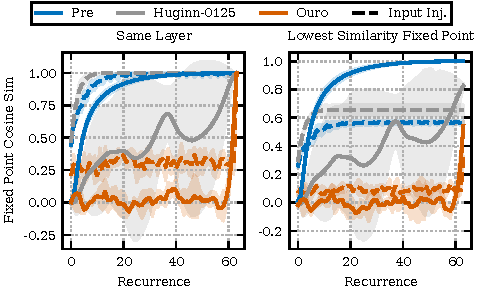
\includegraphics{figures/fixed_point/summarised_stability.pdf}
    \vspace{-0.4cm}
    \caption{\textbf{Cosine similarity between residual streams after each layer and the approximate fixed point} for a range of norms, with and without input injection. Each model is randomly initialized with 12 layers. Cosine similarity is taken between the residual stream after the first layer at each recurrence and \textbf{left:} the approximate fixed point of the first layer, \textbf{right:} the approximate fixed point of the layer with the \emph{lowest} cosine similarity to the first layer.}
    \vspace{-0.3cm}
    \label{fig:summarised_stability}
\end{figure}

\section{Stages of Inference in Looped Models Mirror Feedforward Computation}\label{sec:stages_of_inference}
The previous section shows that, empirically, a wide range of models converge to a regime in which attention patterns within individual layers change only minimally across recurrences. As a result, attention dynamics in looped Transformers are constrained in depth, since layers are cyclically weight-tied to earlier ones. This behavior contrasts with feedforward Transformers, which impose no such constraints and exhibit sharp, layer-wise changes in attention patterns across depth. Prior work has linked these sharp transitions to characteristic stages of inference \citep{lad2024remarkable,queipo2025attention}, introduced in \Cref{subsec:stages_of_inference_prelim}. In this section, we study how cyclic weight sharing alters these stages of inference in looped Transformers. In the main text we frame our analysis using \emph{ColSum concentration}, a metric for identifying stages of inference introduced in \Cref{subsec:stages_of_inference_prelim}, with extensive additional results in \Cref{appen:cyclic_soi}.

% The previous section demonstrates that empirically, a range of models tend towards a state in which the attention patterns of individual layers change very little between recurrences. This limits the extent to which attention patterns can change in depth, as they are cyclically weight-tied with previous layers: this stands in contrast to behavior in feedforward Transformers, which have no such restrictions and in which sharp changes are empirically observed between attention patterns throughout the depth of the Transformer. These attention patterns have been linked to characteristic stages of inference \citep{lad2024remarkable,queipo2025attention} -- introduced in \Cref{subsec:stages_of_inference_prelim} -- which similarly exhibit sharp changes in depth. In this section, we examine how cyclic weight-sharing impacts stages of inference in looped Transformers. We communicate our findings through the lens of colsum concentration, a characteristic measurement of stages of inference introduced in \Cref{subsec:stages_of_inference_prelim}, and we include extensive additional results in \Cref{appen:cyclic_soi} to back up our claims. 

We visualize ColSum concentration over the realized depth of Retrofitted Llama in \Cref{fig:stages_of_inference_cyclic_and_similar}, revealing consistent mixing cycles that repeat with every iteration of the recurrent block. However, \emph{each individual layer} (solid colorful lines) changes very little in realized depth: after an initial transitory phase they quickly converge towards constant behavior.

\begin{figure}[ht]
    \centering    
    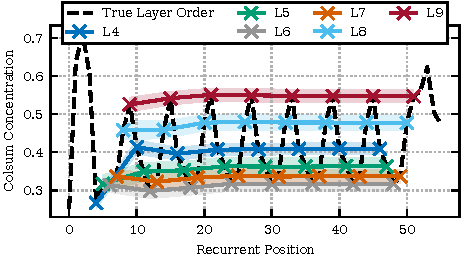
\includegraphics{figures/stages_of_inference/similar_behaviour/similar_behaviour_summarised.pdf}
    \vspace{-0.4cm}
    \caption{\textbf{Stages of inference for retrofitted Llama \citep{mcleish2025teaching} with 8 recurrences.} Individual layers are visualized as solid lines; successive layers in the looped Transformer as a dashed black line. Individual layers quickly converge towards constant behavior, and the cyclic action of these layers results in cyclic stages of inference.}
    \vspace{-0.3cm}
    \label{fig:stages_of_inference_cyclic_and_similar}
\end{figure}

Instead of occurring throughout the realized depth of the looped model, we find that the familiar feedforward stages of inference occur \emph{within} each looped block. \Cref{fig:summarised_recurrent_block_stages} demonstrates that ColSum concentration within each looped block closely resembles that of feedforward models. We draw attention to two observations: 1) Ouro 1.4B, despite being trained \emph{from scratch} with recurrence, mirrors Llama mixing stages and 2) the retrofitted models closely follow the stages of inference of their associated base model, but the initial and final stages are performed only once by the prelude and coda respectively, while the ``middle'' stages are repeated in the recurrent block. It is particularly remarkable that these stages of inference appear in each \ouro{} recurrent block when pretraining from initialization; we discuss further the formation of stages of inference, and attempt to isolate their formation from specific training procedures, in \Cref{sec:self_organising_soi}.

\begin{figure*}[ht]
    \centering    
    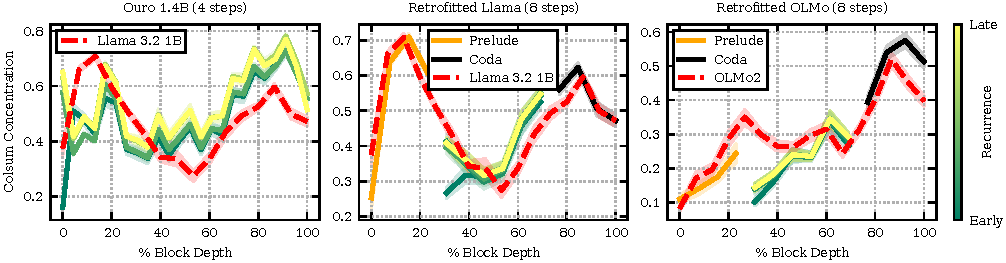
\includegraphics[width=0.9\linewidth]{figures/stages_of_inference/recurrent/summarised.pdf}
    \vspace{-0.1cm}
    \caption{\textbf{Stages of inference for each recurrent loop in} \textbf{left:} Ouro 1.4B \citep{zhu2025scaling} \textbf{center:} retrofitted Llama and \textbf{right}: retrofitted OLMo \citep{mcleish2025teaching}. Ouro 1.4B resembles Llama stages of inference, and the two retrofitted to their associated base models.}
    \vspace{-0.5cm}

    \label{fig:summarised_recurrent_block_stages}
\end{figure*}



However, \raven{} does \emph{not} demonstrate clear stages of inference (\Cref{fig:raven_recurrent_block_stages}). We suggest that this is likely due to the specific norm structures used by these models (\Cref{tab:looped_model_details}). \raven{} and \ouro{} both use a ``sandwich'' norm structure, but \raven{} implements this by normalizing the residual streams whereas \ouro{} instead normalizes the outputs of the attention and MLP units, only normalizing the residual stream at the end of each recurrent block. We demonstrate the impact of the different norms by plotting residual stream magnitudes for a range of models in \Cref{fig:residual_norm_comparison}. This means that \raven{} is unable to develop the growth in residual stream magnitude that \citet[Section 3.3]{queipo2025attention} note \emph{causes} compression behavior, leading to sink formation and stages of inference.


\begin{figure}[ht]
    \centering
    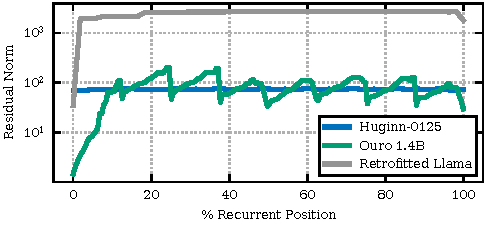
\includegraphics{figures/stages_of_inference/residual_norm_comparison.pdf}
    \vspace{-0.9cm}
    \caption{\textbf{Norms of the residual stream for a range of models,} demonstrating that \raven{} is unable to develop the activation magnitude changes required for stages of inference due to its repeated normalization of the residual stream.}
    % \vspace{-0.6cm}
    \label{fig:residual_norm_comparison}
\end{figure}



\begin{figure*}[!t]
    \centering
    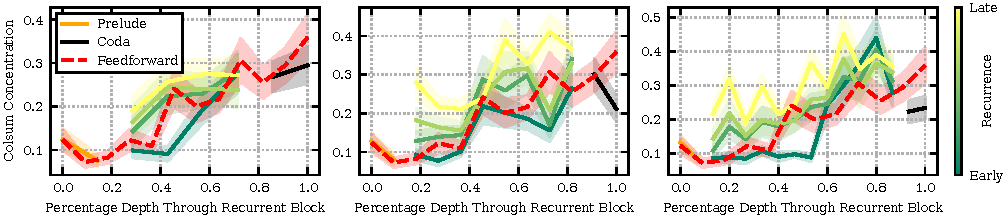
\includegraphics[width=0.9\linewidth]{figures/training/summary.pdf}
    \vspace{-0.4cm}
    \caption{\textbf{ColSum concentrations for small-scale trained Looped Transformers with a simplified loss function and constant train recurrence schedule of 4 recurrences}. Also visualized in red is a ``control'' feedforward Transformer of depth 12. All models have 2 prelude and 2 coda layers with no input injection, \textbf{left:} 4 recurrent layers, \textbf{center:} 8 recurrent layers, \textbf{right:} 12 recurrent layers.}
    \label{fig:summary_training_stages_of_interest}
\end{figure*}

\subsection{Self-Organization Into Stages of Inference}\label{sec:self_organising_soi}
An open question from our analysis of pretrained models (\Cref{fig:summarised_recurrent_block_stages}) is whether stages of inference emerge naturally during pretraining, or whether they are instead induced by specific aspects of the training procedure. Several mechanisms may introduce an implicit bias toward feedforward stages of inference: retrofitted models \citep{mcleish2025teaching} may inherit the inference stages of the underlying base model; models trained with recurrence schedulers that permit a single recurrence \citep{geiping2025scaling,mcleish2025teaching} are partially optimized as feedforward models; training objectives that decompose into separate loss terms for each recurrence \citep{zhu2025scaling} partially correspond to feedforward model training.



% One question unanswered by our analysis of pretrained models (\Cref{fig:summarised_recurrent_block_stages}) is whether stages of inference emerge naturally when pretraining or if they must ``induced'' by some other aspect of the training procedure. There are multiple ways we suggest that this bias towards feedforward stages of inference may be introduced:
% \begin{itemize}
%     \item Any retrofitted model \citep{mcleish2025teaching} may inherit the stages of inference of the underlying base model.
%     \item Any model trained with a recurrence scheduler that allows for single recurrence is trained -- in part -- as a straightforward feedforward model, potentially biasing the formation of stages of inference. This is the case for \citet{geiping2025scaling,mcleish2025teaching}.
%     \item If the loss function is a sum of separate components for each recurrence, then a component of the loss is simply that of a feedforward model. This is the case for \citet{zhu2025scaling}.
% \end{itemize}

Therefore in this section we seek to investigate whether stages of inference can arise in Looped Transformers \emph{without} these training biases. To explore this we pre-train several small-scale Looped Transformers, explicitly removing the biases above: we pre-train from scratch with a constant recurrence of 4, using a standard loss that considers only the final latent state when predicting the next token. Our code and training procedure are adapted from \citet{nanochat}; additional details can be found in \Cref{appen:experiment_details}.

ColSum concentrations for these trained Looped Transformers with configurations $(2, 4\otimes 4, 2)$, $(2, 8\otimes 4, 2)$ and $(2, 12\otimes 4, 2)$ are plotted in \Cref{fig:summary_training_stages_of_interest}. We compare these to a ``control'' feedforward network without recurrence, of depth 12. These experiments are on a small scale and as such need to be treated with caution. However, they appear to provide initial evidence that -- even without training methods that may bias towards feedforward stages of inference -- looped models have a tendency to \emph{self-organize} into multiple different mixing stages in recurrent depth, which resemble feedforward stages. The fact that the optimization of these models results in these mixing stages of inference suggests that they are beneficial to language modeling even when applied repeatedly in recurrent depth. We additionally test the impact of input injection and sandwich layers in \Cref{appen:architecture_stages_of_inference}.



\subsection{Stability to Unseen Numbers of Recurrences}\label{sec:stability}

\Cref{sec:cyclic_similarity} establishes that some looped Transformer architectures converge to a fixed point (such as the retrofitted series and \raven{}) while others do not (such as Ouro). However, when evaluating these looped Transformers within the range of recurrences on which they were trained (\Cref{sec:stages_of_inference}), we see extremely similar behavior: convergence to feedforward stages of inference within each recurrent block.

In this section, we demonstrate that a significant difference arises when generalizing to unseen test-time recurrence depths: models that do not reach a fixed point exhibit \textbf{unstable stages of inference}. Conversely, models with recurrent-block-wise stages of inference that also converge to a fixed point are guaranteed to keep enacting these stages of inference for arbitrary test time recurrences.

We first verify this stability in \Cref{fig:stability_in_total_recurrence}, an extended plot of \Cref{fig:stages_of_inference_cyclic_and_similar}. This demonstrates that for retrofitted Llama (results hold for other models using input injection), each individual layer quickly reaches a stable states and then exhibits consistent stages of inference behavior for an arbitrary number of test time recurrences. However, Ouro 1.4B does not exhibit this behavior, with individual layers changing continuously throughout later recurrences. The effect that this has on stages of inference is visualized in \Cref{fig:stability_in_percentage_depth}.
\begin{figure}[ht]
    \centering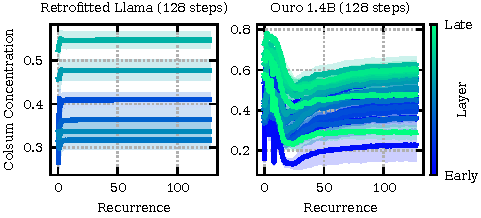
\includegraphics{figures/stages_of_inference/similar_behaviour/stability_in_total_recurrence_summarised.pdf}
    \vspace{-0.4cm}
    \caption{\textbf{Colsum concentration of each layer} with successive recurrences for \textbf{left:} retrofitted Llama and \textbf{right:} Ouro 1.4B, both using 128 recurrences. While the layers of retrofitted Llama quickly converge to constant ColSum concentration, the layers of Ouro continually change throughout the recurrences tested.}
    \label{fig:stability_in_total_recurrence}
\end{figure}
\begin{figure}[ht]
    \centering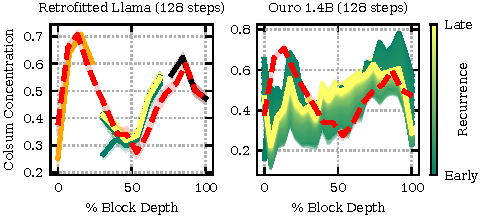
\includegraphics{figures/stages_of_inference/similar_behaviour/stability_in_percentage_depth_summarised.pdf}
    \vspace{-0.3cm}
    \caption{\textbf{Colsum concentration of each layer vs the percentage depth at which that layer appears in the recurrent block.} \textbf{Left:} retrofitted Llama and \textbf{right:} Ouro 1.4B, both using 128 recurrences. Feedforward Llama shown in dashed red.}\label{fig:stability_in_percentage_depth}
\end{figure}

 Existing research implies that this stability correlates with out-of-domain performance. Models which exhibit ``stable'' stages of inference for arbitrary test time iterations also \emph{avoid performance deterioration} in this extrapolation regime: whereas extrapolation beyond training recurrences harms the performance of \ouro{} \citep[Tab. 10]{zhu2025scaling}, \raven{} performance remains constant in this extrapolation region \citep[Fig. 1]{geiping2025scaling}.

\section{Conclusion}\label{sec:conclusion}

This paper examines the limiting behavior of Looped Transformers, exploring implications for ``mixing'' stages of inference observed in feedforward models. We demonstrate across a range of architectures that recurrent blocks tend to ``mirror'' the stages of a feedforward Transformer, and provide evidence that this may be emergent behavior learned during training, even when not explicitly encouraged by the training process. We further investigate the implications for these mixing stages when models converge to a stable fixed point, and when they do not.

\paragraph{Implications of Findings}

The implications of our findings are bidirectional. On the one hand, the structure of looped architectures provides a novel lens to study stages of inference, while tracking these stages simultaneously reveals the internal mechanics of recurrent depth. In particular, since looped models decouple functional depth from parameter count, they provide an interesting new perspective on \emph{why} these stages of inference form: previous work had suggested that these stages exist to mitigate the ``harms'' of transformer depth \citep{barbero2025llms,queipo2025attention}, however our work shows that looped models develop these same stages while simultaneously improving performance with greater recurrent depth. On the other hand, our findings that looped models exhibit (and self-organize into) similar stages of inference to feedforward models means that insights from the feedforward setting can be applied to looped models: predictable stages offer actionable pathways for efficient architectural design, including stage-dependent attention sparsification and the leaner parameterization of middle-stage MLPs where representations are reliably compressed and low-rank.

\paragraph{Limitations and Future Work}

We focus exclusively on cyclic recurrence as this appears to be the dominant approach in the literature. However, this means our analysis does not extend to sequential recurrence with multiple separate recurrent blocks; for analysis of this setting we refer the reader to \citet{pappone2025two}. Despite empirically investigating the architectural choices that result in stable limiting behavior in looped models, we have not established analytically why this is the case, nor whether this stable limiting behavior is desirable or restrictive for reasoning tasks.

\clearpage
\section*{Impact Statement}

Ethical aspects and future societal consequences of this particular work are limited. The goal of our work is to advance understanding of looped Language Models, which themselves seem to demonstrate strong reasoning performance; as such, our work is in support of a field that has potential societal consequences if future models are able to undertake more advanced reasoning tasks. However, we do not within this work introduce any more powerful reasoning models, and the impact of our work is limited to understanding existing models, and potentially guiding future advancements.

\section*{Acknowledgments}

HB acknowledges funding support from the EPSRC Centre for Doctoral Training in Autonomous Intelligent Machines and Systems No. EP/S024050/1. MB is partially supported by the EPSRC Turing AI World-Leading Research Fellowship No. EP/X040062/1 and EPSRC AI Hub No. EP/Y028872/1.


\bibliography{looped_llms}
\bibliographystyle{icml2025}


%%%%%%%%%%%%%%%%%%%%%%%%%%%%%%%%%%%%%%%%%%%%%%%%%%%%%%%%%%%%%%%%%%%%%%%%%%%%%%%
%%%%%%%%%%%%%%%%%%%%%%%%%%%%%%%%%%%%%%%%%%%%%%%%%%%%%%%%%%%%%%%%%%%%%%%%%%%%%%%
% APPENDIX
%%%%%%%%%%%%%%%%%%%%%%%%%%%%%%%%%%%%%%%%%%%%%%%%%%%%%%%%%%%%%%%%%%%%%%%%%%%%%%%
%%%%%%%%%%%%%%%%%%%%%%%%%%%%%%%%%%%%%%%%%%%%%%%%%%%%%%%%%%%%%%%%%%%%%%%%%%%%%%%
\newpage
\appendix
\onecolumn

\etocdepthtag.toc{appendix}
\etocsettocstyle{\section*{Appendix Contents}}{} % Title of the TOC
\setcounter{tocdepth}{3}
\etocsettagdepth{mtoc}{none}           % Hide main text sections
\etocsettagdepth{appendix}{subsection}  % Show appendix sections (adjust depth as needed)
\tableofcontents                        % Print the TOC



% \section{Fixed Point, Limiting Behavior and Path Independence}

% In the looped Transformer and other related literature, several concepts are frequently discussed that pertain to 

\newpage

% Temporarily remove this for arxiv version. Make sure this comes back.
% \section{Impact of Input Injection}

% \input{sections/appendices/inp_inj_theory.tex}

\section{Proofs of Propositions}
\paragraph{Proof of \Cref{prop:cyclic_fixed_point}}

\begin{sketch}
    Note
    $$\stack_k(\mX') = \block_k(\block_{k-1}( \dots \block_1(\mX') \dots )) = \mX'$$
    Applying $\block_1$ to both sides yields to
    $\block_1(\block_k(\block_{k-1}( \dots \block_1(\\\mX') \dots ))) = \block_1(\mX').$
    Defining $\mY' = \block_1(\mX')$, we obtain
    $\block_1(\block_k(\block_{k-1}( \dots \block_2(\mY') \dots ))) = \mY'$. 
    The general proof follows by induction, and extends trivially to input injection.   
\end{sketch}

\begin{proof}
    Assume that $(l,k)$-Recurrent block $S_k$ reaches a fixed point such that $S_k(\mX') = \mX'$. Note that
    $$\stack_k(\mX') = \block_{k-1}(\block_{k-2}( \dots \block_0(\mX') \dots )) = \mX'$$
    define the cyclic shift function $f_n(i) = (i + n) \mod k$. Now we aim to prove by induction
    $$\forall n \in \mathbb{Z}_+ \cup \{0\} : \block_{f_n(k-1)}(\block_{f_n(k-2)}( \dots \block_{f_n(0)}(\mZ') \dots )) = \mZ'$$
    for some $\mZ'$. The base case $n=0$ is trivial as $\forall i < k: f_0(i) = i$.
    Now assume for some $n=j$
    \begin{equation}\label{eq:ind_hyp}
        \block_{f_j(k-1)}(\block_{f_j(k-2)}( \dots \block_{f_j(0)}(\mZ') \dots )) = \mZ'
    \end{equation}
    Now, let $n=j+1$. Note 
    $$f_{j+1}(i) = (i + j + 1) \mod k = f_{j}(i + 1)$$
    Therefore
    \begin{align}
        \block_{f_{j+1}(k-1)}(\block_{f_{j+1}(k-2)}( \dots \block_{f_{j+1}(0)}(\mY) \dots )) &= \block_{f_j(k)}(\block_{f_j(k-1)}( \dots \block_{f_j(1)}(\mY) \dots )) \\
        &= \block_{f_j(0)}(\block_{f_j(k-1)}( \dots \block_{f_j(1)}(\mY) \dots ))  \label{eq:cycle_applied}
    \end{align}
     Now take \Cref{eq:ind_hyp} and apply $\block_{f_j(0)}$ to both sides, defining a new fixed point $\mZ^{\prime \prime} = \block_{f_j(0)}(\mZ')$:
     \begin{align}
         \block_{f_j(0)}(\block_{f_j(k-1)}(\block_{f_j(k-2)}( \dots \block_{f_j(0)}(\mZ') \dots ))) &= \block_{f_j(0)}(\mZ') \\
         \block_{f_j(0)}(\block_{f_j(k-1)}(\block_{f_j(k-2)}( \dots \block_{f_j(1)}(\mZ^{\prime \prime}) \dots ))) &= \mZ^{\prime \prime} \label{eq:new_fixed_point}
     \end{align}
     Combining \Cref{eq:new_fixed_point} and \Cref{eq:cycle_applied}, we see that there exists a fixed point $\mZ^{\prime \prime}$ such that
     $$\block_{f_{j+1}(k-1)}(\block_{f_{j+1}(k-2)}( \dots \block_{f_{j+1}(0)}(\mZ^{\prime \prime}) \dots )) = \mZ^{\prime \prime}$$
     Therefore completing the induction step and proving the proposition.
\end{proof}

\paragraph{Proof of \Cref{prop:similar_attention_patterns}}
\begin{proof}
Define
$$\mathcal S_\ell(\mX):=\softmax(A_\ell(\mX)) = \softmax{\left ( \frac{\mX \mW_Q \mW_K^{\top} \mX^{\top}}{\sqrt{d}} \right )}$$
Let $L_{\mathrm{sm}}$ be the Lipschitz constant of the row-wise softmax such that
    \begin{equation}\label{eq:softmax_lip}
        \big\|\mathcal S_\ell(\mX_{\ell,t})-\mathcal S_\ell(\mX_{\ell,t-1})\big\| \leq L_{\mathrm{sm}} \big\| A_\ell(\mX_{\ell,t})- A_\ell(\mX_{\ell,t-1})\big\|
    \end{equation}
    Recently \citet{nair2025softmax} shows that $L_{\mathrm{sm}} = 1/2$.

    Define for convenience $\mM = \mW_Q \mW_K^{\top}$ and $\Delta_{\ell, t} = \mX_{\ell,t}- \mX_{\ell,t-1}$. Then
    \begin{align*}
        A_\ell(\mX_{\ell,t})- A_\ell(\mX_{\ell,t-1}) &= \frac{\mX_{\ell,t} \mW_Q \mW_K^{\top} \mX^{\top}_{\ell,t}}{\sqrt{d}} - \frac{\mX_{\ell,t-1} \mW_Q \mW_K^{\top} \mX^{\top}_{\ell,t-1}}{\sqrt{d}} \\
        &= \frac{1}{\sqrt{d}} \left ( \left ( \Delta_{\ell, t} + \mX_{\ell, t-1} \right ) \mM \left ( \Delta_{\ell, t} + \mX_{\ell, t-1} \right )^{\top} - \mX_{\ell,t-1} \mM \mX^{\top}_{\ell,t-1} \right ) \\
        &= \frac{1}{\sqrt{d}} \left (  {\Delta_{\ell, t} \mM \Delta_{\ell, t}^{\top}} + \Delta_{\ell, t} \mM \mX_{\ell, t-1}^{\top} +  \mX_{\ell, t-1} \mM \Delta_{\ell, t}^{\top} + \cancel{\mX_{\ell, t-1} \mM \mX_{\ell, t-1}^{\top}} - \cancel{\mX_{\ell,t-1} \mM \mX^{\top}_{\ell,t-1}} \right )  \\
        &= \frac{1}{\sqrt{d}} \left (  \Delta_{\ell, t} \mM \left ( \Delta_{\ell, t} + \mX_{\ell, t-1} \right )^{\top} +  \mX_{\ell, t-1} \mM \Delta_{\ell, t}^{\top} \right ) \\
        &= \frac{1}{\sqrt{d}} \left (  \Delta_{\ell, t} \mM \mX_{\ell, t}^{\top} +  \mX_{\ell, t-1} \mM \Delta_{\ell, t}^{\top} \right ) \\
    \end{align*}
    Therefore,
    \begin{align*}
        \big\|A_\ell(\mX_{\ell,t})- A_\ell(\mX_{\ell,t-1})\big\| &= \big\| \frac{1}{\sqrt{d}} \left (  \Delta_{\ell, t} \mM \mX_{\ell, t}^{\top} +  \mX_{\ell, t-1} \mM \Delta_{\ell, t}^{\top} \right ) \big\| \\
        &\leq \frac{1}{\sqrt{d}} \left ( \big\| \Delta_{\ell, t} \mM \mX_{\ell, t}^{\top} \big\| + \big\| \mX_{\ell, t-1} \mM \Delta_{\ell, t}^{\top} \big\| \right ) \\
        &\leq \frac{\big\| \mM \big\| \left ( \big\| \mX_{\ell, t} \big\| + \big\| \mX_{\ell, t-1} \big\| \right )}{\sqrt{d}} \big\| \Delta_{\ell, t} \big\|
    \end{align*}
    Assuming $\|\mX_{\ell,t}\|\le B$ for all $t$, and defining $\kappa_\ell = \|\mW_{Q,\ell}\mW_{K,\ell}^\top\| = \big\| \mM \big\|$, we see
    \begin{equation}\label{eq:a_inequality}
        \big\|A_\ell(\mX_{\ell,t})- A_\ell(\mX_{\ell,t-1})\big\| \leq \frac{2 B \kappa_\ell}{\sqrt{d}} \big\|\mX_{\ell,t}-\mX_{\ell,t-1}\big\|
    \end{equation}
    Combining \Cref{eq:softmax_lip} and \Cref{eq:a_inequality}, we complete the proof:
    \begin{equation}
        \big\|\mathcal S_\ell(\mX_{\ell,t})-\mathcal S_\ell(\mX_{\ell,t-1})\big\| \leq L_{\mathrm{sm}} \frac{2 B \kappa_\ell}{\sqrt{d}} \big\|\mX_{\ell,t}-\mX_{\ell,t-1}\big\|
    \end{equation}
\end{proof}

\section{Additional Experimental Details}\label{appen:experiment_details}

Unless stated otherwise, all of our experiments are averaged over the same subset of 256 random examples from the test split of the GSM8k \citep{cobbe2021gsm8k} dataset. A few illustrative plots (for example, latent space trajectories) are instead produced with a \emph{test sequence} that we obtain from \citet{barbero2025llms}: ``Hello! I've been well. I hope that you're doing well.'' Additional results targetting non-reasoning behavior using the HellaSwag dataset (following an identical setup of running inference on the same 256 random examples from the test split) can be found in \Cref{appen:hellaswag_soi}.

All pretrained models are obtained from Huggingface, model references provided in \Cref{tab:model_ids_and_bases}. We use standard settings for the tokenizers of each model, and as such some models prepend a BOS token whereas others do not: we make this clear in the `Prepends BOS' column of the same table.

\begin{table*}[ht]
    \centering
    \caption{{Looped Transformer architecture summary.} Retrofitted Llama and OLMo use 6 layers in their recurrent block, TinyLlama uses 8.}
    \label{tab:looped_model_details}
    \begin{tabularx}{\textwidth}{Xcccc}
        \toprule
        \textbf{Model Name} & \textbf{Structure} & \textbf{Train Loops} & \textbf{Block Norm} & \textbf{Norm After Loop?} \\
        \midrule
        Ouro 1.4B \citep{zhu2025scaling} & $(0,24,0)$ & 4 & $\begin{aligned}
            \hat{\mX} &=  \mX + n \left (\attn(n(\mX) \right ) \\
    {\mX}' &=  \hat{\mX} + n \left (\text{MLP}(n(\hat{\mX})) \right ) \\
        \end{aligned}$ & Yes \\ \midrule
        \raven{} \citep{geiping2025scaling} & $(2,4,2)_I$ & 32 & $\begin{aligned}
            \hat{\mX} &= n \left ( \mX + \attn(n(\mX) \right ) \\
    {\mX}' &= n \left ( \hat{\mX} + \text{MLP}(n(\hat{\mX})) \right )
        \end{aligned}$ & Yes \\ \midrule
        Retrofitted \citep{mcleish2025teaching} & $(4,6,4)_I$ / $(4,8,4)_I$ & 32 & $\begin{aligned}
            \hat{\mX} &= \mX + \attn(n(\mX) \\
    {\mX}' &= \hat{\mX} + \text{MLP}(n(\hat{\mX})) 
        \end{aligned}$ & No \\
        \bottomrule
    \end{tabularx}
\end{table*}

\begin{table}[h!]
\centering
\begin{tabularx}{\textwidth}{|c|c|X|X|c|X|}
\hline
\textbf{Model} & \textbf{Num Params} & \textbf{Huggingface ID} & \textbf{Base Model} & \textbf{Prepends BOS} & \textbf{Notes} \\ \hline
\ouro{} 1.4B & 1.4B & \path{ByteDance/Ouro-1.4B} & - & $\cross$ & - \\ \hline
\ouro{} 2.6B & 2.6B & \path{ByteDance/Ouro-2.6B} & \path{ByteDance/Ouro-1.4B} & $\cross$ & ``Upcycled'' from \ouro{} 1.4B by repeating the same layers after the first training phase. \\ \hline 
\raven{} & 3.5B & \path{tomg-group-umd/huginn-0125} & - & $\checkmark$ & - \\ \hline
Retrofitted Llama & 1B & \path{smcleish/Recurrent-Llama-3.2-train-recurrence-32} & \path{meta-llama/Llama-3.2-1B} & $\checkmark$ & Models trained with fewer recurrences exhibit similar mixing patterns. \\ \hline
Retrofitted OLMo-2 & 1B & \path{smcleish/Recurrent-OLMo-2-0425-train-recurrence-32} & \path{allenai/OLMo-2-0425-1B} & $\cross$ & As above. \\  \hline
Retrofitted TinyLlama & 0.8B & \path{smcleish/Recurrent-TinyLlama-3T-train-recurrence-32} & \path{TinyLlama/TinyLlama-1.1B-intermediate-step-1431k-3T} & $\checkmark$ & As above. \\  \hline
\end{tabularx}
\caption{Additional Huggingface details on pretrained Looped models used.}
\label{tab:model_ids_and_bases}
\end{table}

Our small training runs in \Cref{sec:self_organising_soi} are performed by adapting a publicly available fork of Nanochat \citep{nanochat}, \url{https://github.com/TrelisResearch/nanochat/tree/recursive}. For all experiments we use a model dimension (residual stream) of 512 (4 heads of dimension 128) and train for 3.7B tokens. As discussed in the main text, loss is the same as that of a regular feedforward model: cross entropy loss on the final output representation (as opposed to the summed loss of \citet{zhu2025scaling}). Each model is trained for a \emph{constant} 4 recurrences (as opposed to the Poisson sampling of \citet{geiping2025scaling}). All models use pre-norm only: this norm does not result in the stability issues reported by \citet{geiping2025scaling,zhu2025scaling}, but this is likely because we are operating at a far smaller scale.

\FloatBarrier
\section{Non-Fixed-Point Limiting Behavior}\label{appen:orbits_and_sliders}
\subsection{How Frequent is Non-Fixed-Point Behavior?}

In this section we investigate more closely the ``orbits'' and ``sliders'' initially observed by \citet{geiping2025scaling}. These are important as they appear to represent stable limiting behavior that are \textbf{not fixed points}.

We develop a heuristic algorithm to detect these behaviors, presented in \Cref{alg:orbit_slider}. We use the sequence of cosine similarities from the final recurrent layer (per token), where the output residual stream after each of 128 recurrences is compared to the final residual stream (as in \Cref{fig:fixed_point_cosine_similarities}). This is visualized in the leftmost column of \Cref{fig:orbit_algorithm_examples}. We set threshold $\tau=0.05$ and fixed-point fraction $\rho=0.9$.

Using this algorithm, we classify the limiting behavior over \emph{all} tokens in the GSM8k test set for the \raven{} and \rllama{} models. We discover that the \emph{system prompt} used before presenting the GSM8k question has a large impact on the limiting behavior types and as such we test the following prompts across both models:
\paragraph{Long Persona} This is the system prompt used by \citet{geiping2025scaling} to produce their Orbit plots:
\begin{tcolorbox}[colback=gray!10, colframe=gray!50, arc=5pt]
You are Huginn, an AI assistant who embodies careful thought and deliberation. Your responses demonstrate:

Methodical reasoning, breaking complex problems into clear steps

Mathematical and programming expertise grounded in fundamentals

The ability to acknowledge uncertainty and correct course when needed

Clear communication that illuminates rather than just informs

When engaging with questions, you first seek to understand their deeper structure before answering. Like your namesake who flew the nine worlds seeking wisdom, you explore problems from multiple angles, helping users build genuine understanding rather than providing shallow answers.
You express warmth and intellectual curiosity while maintaining professionalism. When faced with errors or confusion, you model honest reflection and careful correction. Your goal is not just to provide answers, but to help humans develop clearer, deeper thinking.
\end{tcolorbox}

\paragraph{Long Persona (Padded)} This is the same prompt as above but with all tokens replaced with the padding token: we include this to test whether the behavior arises purely due to the length of the input.

\paragraph{Short Math} This is the system prompt used by \citet{geiping2025scaling} in their GSM8k benchmark evaluation:
\begin{tcolorbox}[colback=gray!10, colframe=gray!50, arc=5pt]
You are a helpful assistant that is capable of helping users with mathematical reasoning.
\end{tcolorbox}

We present the percentage of GSM8k tokens that exhibit each classification of limiting behavior in \Cref{tab:behavior_tokens} and the percentage of GSM8k examples that exhibit each classification of limiting behavior \emph{across any of their tokens} in \Cref{tab:behavior_existence}.

These results reveal that these non-fixed-point limiting behaviors appear to be extremely rare in practice: without a system prompt (the setting used throughout this paper) only approximately 0.02\% of tokens exhibit non-fixed-point behavior. This percentage can be significantly increased with the longer system prompt, but these behaviors remain rare at 0.14\%. Curiously, the ``Persona'' system prompt used by \citet{geiping2025scaling} seems to increase the occurrence of these orbits and sliders more than a comparable prompt of padding tokens, suggesting that the effect is not purely to do with sequence length.

We highlight that these exact results need to be treated with caution: the absolute values vary significantly depending on the algorithm hyperparameters chosen, and in the absence of a good external metric we selected these hyperparameters manually via visual inspection of the trajectories and cosine similarities to ensure the results agreed with intuition. However, across different hyperparameters the results consistently showed that non-fixed-point behavior is rare and that the long persona prompt results in a greater rate of non-fixed-point behavior. We leave in-depth classification and explanation of this phenomena to future work.

\begin{algorithm}
\caption{Per-token limiting behaviour classification}\label{alg:orbit_slider}
\begin{algorithmic}[1]
\REQUIRE similarity (or norm) series $\mathbf{s} \in \mathbb{R}^{n}$ for one token
         over the last $n$ recurrent firings (final firing excluded);
         threshold $\tau$; fixed-point fraction $\rho$
\ENSURE  Label $\ell \in \{\textsc{FixedPoint},\, \textsc{Orbit},\, \textsc{Slider},\, \textsc{Unknown}\}$

\STATE \textit{--- Detrend ---}
\STATE Fit linear trend: $[\hat{a},\hat{b}] \gets \arg\min_{a,b}\sum_i (s_i - a i - b)^2$
\STATE $\tilde{\mathbf{s}} \gets \mathbf{s} - (\hat{a}\,\mathbf{t} + \hat{b})$
       \hfill $\triangleright$ $\mathbf{t} = [0, 1, \dots, n-1]^\top$

\STATE \textit{--- Spectral amplitude ---}
\STATE $\mathbf{w} \gets \tilde{\mathbf{s}} \odot \operatorname{Hann}(n)$
       \hfill $\triangleright$ reduce spectral leakage
\STATE $\mathbf{M} \gets |\operatorname{RFFT}(\mathbf{w})|_{1:}$
       \hfill $\triangleright$ discard DC bin
\STATE $k^* \gets \arg\max_k M_k$
\STATE $A \gets 4\, M_{k^*} / n$
       \hfill $\triangleright$ Hann-corrected amplitude

\STATE \textit{--- Classify (first match wins) ---}
\STATE $n_{\text{close}} \gets \#\{i : s_i \geq 1 - \tau\}$
       \hfill $\triangleright$ (or $s_i \leq \tau$ for norm)
\IF{$n_{\text{close}} \geq \rho\, n$}
    \STATE \textbf{return} $\textsc{FixedPoint}$
\ENDIF
\STATE \hfill $\triangleright$ peak-to-peak $= 2A \geq \tau$; at least 2 full cycles in window
\IF{$A \geq \tau/2$ \textbf{ and } $(k^*+1)/n \geq 2/n$}
    \STATE \textbf{return} $\textsc{Orbit}\!\left(\text{freq} = (k^*+1)/n,\; \text{amp} = A\right)$
\ENDIF
\STATE $g \gets \hat{a}$
       \hfill $\triangleright$ linear-fit slope; negate for norm series
\STATE \hfill $\triangleright$ sim increases by ${\geq}\,\tau$ over the full window
\IF{$g > \tau / n$}
    \STATE \textbf{return} $\textsc{Slider}(g)$
\ENDIF
\STATE \textbf{return} $\textsc{Unknown}$
\end{algorithmic}
\end{algorithm}

\begin{figure}
    \centering
    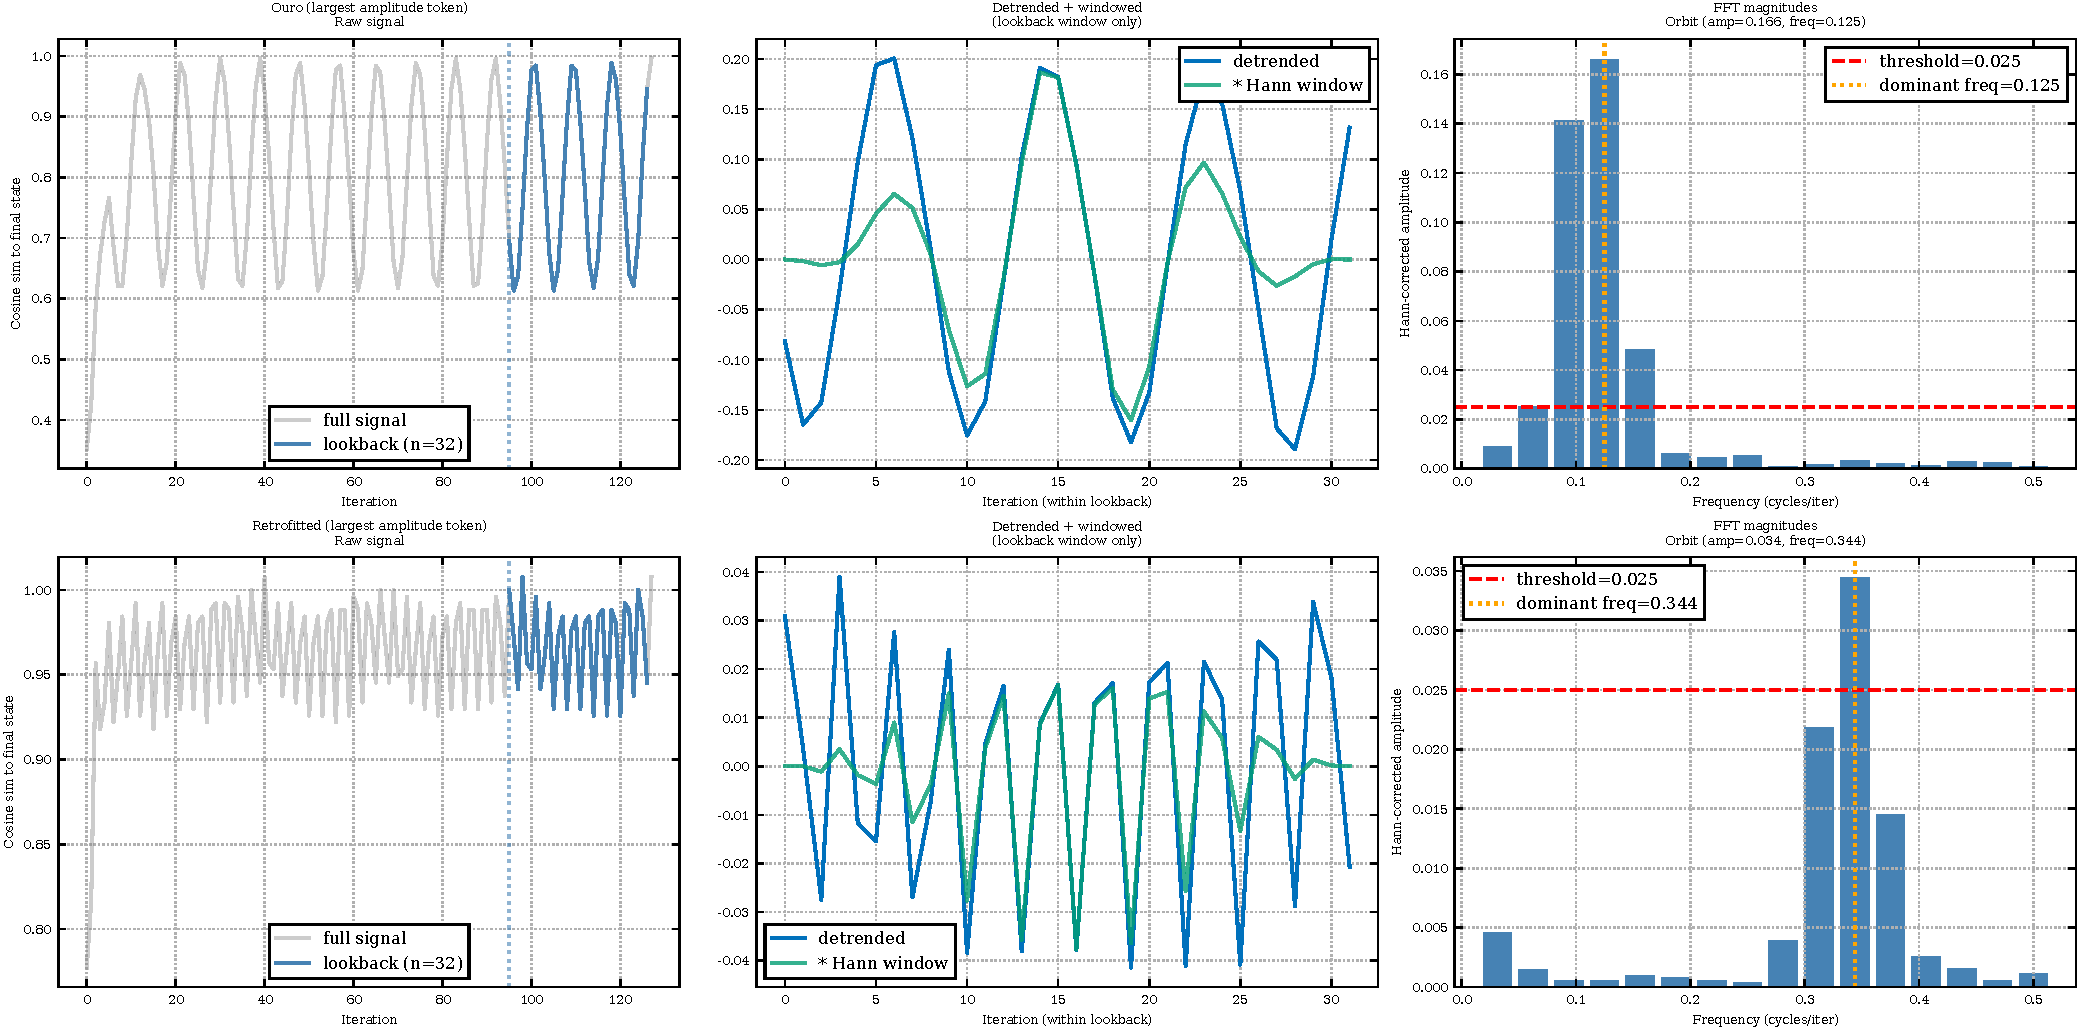
\includegraphics[width=\linewidth]{figures/orbits_sliders/orbit_algorithm_examples.pdf}
    \caption{Visualizing the component parts of the Orbit detection algorithm of \Cref{alg:orbit_slider}. The input sequence (cosine similarities for the residual streams of a given token and layer and successive recursions, as compared to their final residual stream) is visualized in the leftmost column. The center column visualizes the effect of windowing and de-trending, and the rightmost column shows the FFT magnitudes. The top row visualizes the detected Orbit with the largest amplitude for the \raven{} model (which occurs with the ``Long Persona'' prompt) and the bottom row visualizes the largest amplitude for the \rllama{} model (which occurs with no system prompt). We note the appearance of complex, multi-frequency oscillation in this latter case.}
    \label{fig:orbit_algorithm_examples}
\end{figure}

\begin{table}
\centering
\caption{Percentage of tokens exhibiting each behavior type, by model and system prompt.}
\label{tab:behavior_tokens}
\begin{tabular}{llrrrr}
\toprule
Model & System Prompt & Non-Fixed-Point \% & Orbit \% & Slider \% & Unknown \% \\
\midrule
Huginn & Long Persona & 0.14 & 0.13 & 0.00 & 0.01 \\
Huginn & Long Persona (Padded) & 0.05 & 0.02 & 0.02 & 0.01 \\
Huginn & No System Prompt & 0.02 & 0.01 & 0.01 & 0.00 \\
Huginn & Short Math & 0.01 & 0.00 & 0.00 & 0.00 \\
Retrofitted-Llama & Long Persona & 0.00 & 0.00 & 0.00 & 0.00 \\
Retrofitted-Llama & Long Persona (Padded) & 0.00 & 0.00 & 0.00 & 0.00 \\
Retrofitted-Llama & No System Prompt & 0.00 & 0.00 & 0.00 & 0.00 \\
Retrofitted-Llama & Short Math & 0.00 & 0.00 & 0.00 & 0.00 \\
\bottomrule
\end{tabular}
\end{table}

\begin{table}
\centering
\caption{Percentage of examples exhibiting each behavior type at least once on any question token, by model and system prompt.}
\label{tab:behavior_existence}
\begin{tabular}{llrrrr}
\toprule
Model & System Prompt & Non-Fixed-Point \% & Orbit \% & Slider \% & Unknown \% \\
\midrule
Huginn & Long Persona & 2.81 & 2.50 & 0.15 & 1.06 \\
Huginn & Long Persona (Padded) & 0.83 & 0.23 & 0.61 & 0.15 \\
Huginn & No System Prompt & 0.76 & 0.53 & 0.15 & 0.08 \\
Huginn & Short Math & 0.45 & 0.38 & 0.08 & 0.00 \\
Retrofitted-Llama & Long Persona & 0.00 & 0.00 & 0.00 & 0.00 \\
Retrofitted-Llama & Long Persona (Padded) & 0.00 & 0.00 & 0.00 & 0.00 \\
Retrofitted-Llama & No System Prompt & 0.08 & 0.08 & 0.00 & 0.00 \\
Retrofitted-Llama & Short Math & 0.00 & 0.00 & 0.00 & 0.00 \\
\bottomrule
\end{tabular}
\end{table}

\FloatBarrier
\subsection{Do Intermediate Layers Exhibit Non-Fixed-Point Behavior?}

\citet{geiping2025scaling} observe orbits and sliders in the latent states after each application of the entire recurrent block. Here we investigate what occurs in the latent states of the intermediate layers within the recurrent block.

We first extend Figure 16 of \citet{geiping2025scaling} (visualizing latent trajectories on a math prompt), visualizing also the trajectories of the intermediate layer residual streams: this can be found in \Cref{fig:intermediate_nfp_behavior}. This demonstrates that in this particular case, where Orbits occur, they also occur in the intermediate layers. This implies -- viewed in realized depth -- latent trajectories exhibiting multi-scale cyclic behavior.

We investigate this across all GSM8k test examples in \Cref{fig:nfp_behavior_conditional_probability} by plotting the conditional probability of observing each behavior on a given token for any layer, given an observation of observing another behavior on that same token. We discover that orbits and sliders do not co-occur across looped layers, but that orbits and sliders both frequently co-occur with fixed point behavior. ``Unknown'' behavior often co-occurs with orbits, which we suggest may be due to mis-classification of the behavior algorithm.

\begin{figure}[ht]
    \centering
    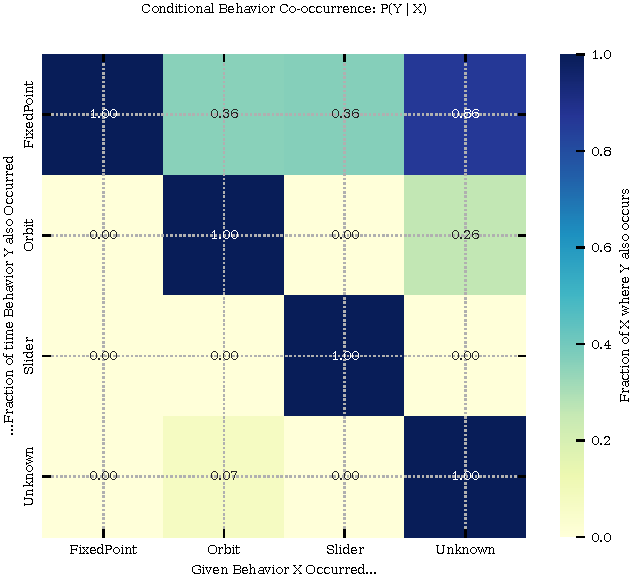
\includegraphics[width=0.6\linewidth]{figures/orbits_sliders/behavior_cooccurrence_heatmap.pdf}
    \caption{Conditional probabilities of co-occurrence for the different limiting behaviors.}
    \label{fig:nfp_behavior_conditional_probability}
\end{figure}

\begin{figure}
    \centering
    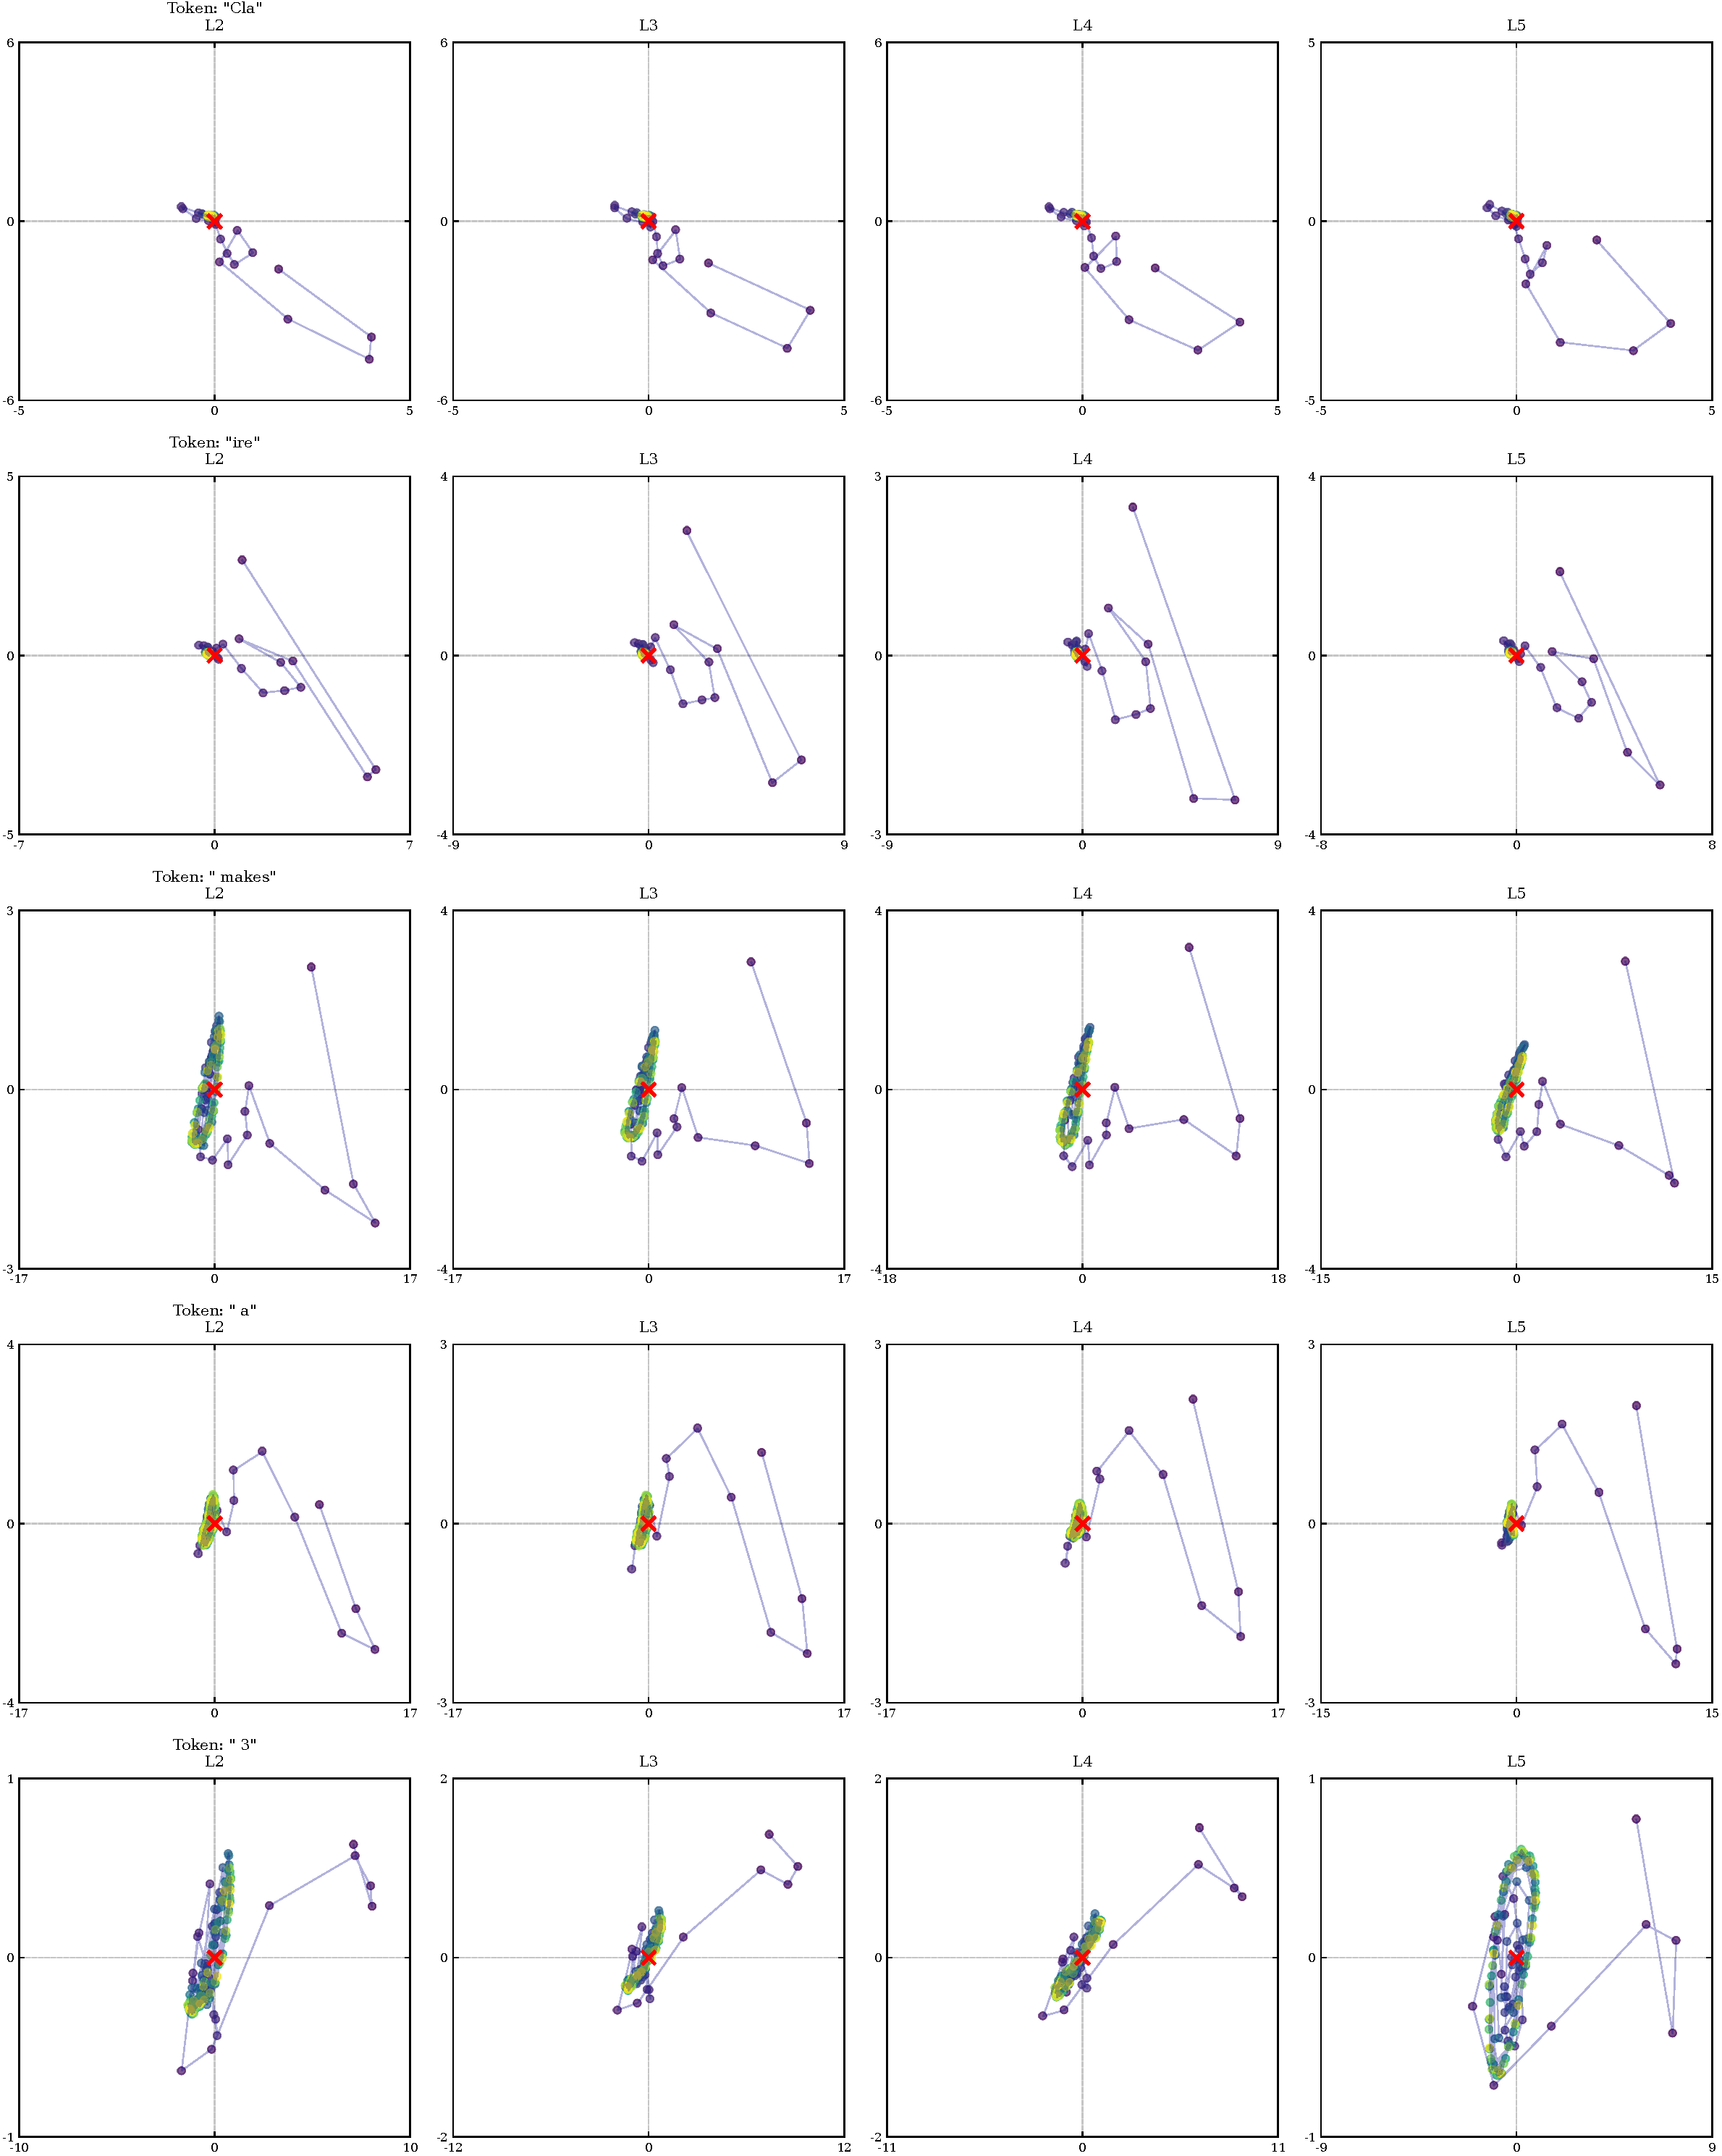
\includegraphics[width=\linewidth]{figures/orbits_sliders/pca_intermediate.pdf}
    \caption{PCA trajectories in the intermediate layers of \raven{}: this reproduces the leftmost column of Fig. 16 in \citet{geiping2025scaling} (the first two principal components) and additionally plots the latent trajectories for the intermediate layers in the recurrent block.}
    \label{fig:intermediate_nfp_behavior}
\end{figure}

\FloatBarrier
\subsection{How Does Non-Fixed-Point Behavior Impact Stages of Inference?}

To complete the link between non-fixed-point behavior and our work we additionally investigate how this behavior impacts the observed stages of inference.

To attempt to isolate the ``worst case'' scenario for stages of inference stability, we plot stages of inference for the GSM8k test prompt that exhibits the greatest orbit amplitude. We first plot in realized depth the extended stages of inference metrics used throughout the paper, see \Cref{fig:orbits_sliders_huginn_stability_in_recurrence}. This demonstrates that sink rates show some variability with the orbiting behavior, but the other metrics remain broadly consistent. We plot also the same metrics in block depth (showing only the final 64 loops) in \Cref{fig:orbits_sliders_huginn_stability_in_depth}: this demonstrates clearly that the stages of inference remain very consistent despite the orbiting behavior.

\begin{figure}[ht]
    \centering
    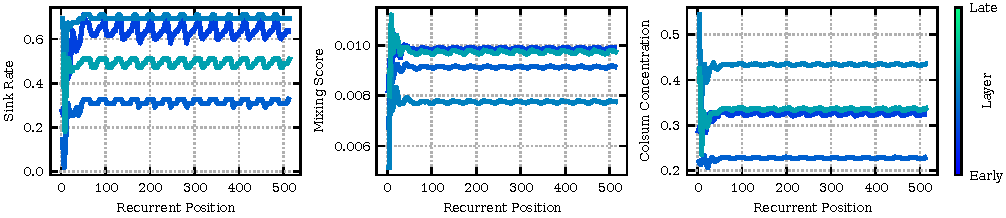
\includegraphics[width=\linewidth]{figures/orbits_sliders/huginn_stability_in_recurrence.pdf}
    \caption{Stages of inference metrics (sink rate, mixing score and colsum concentration) for \raven{} across 128 recurrences, for the GSM8k test prompt that exhibited the largest orbit amplitude. Visualized in realized depth.}
    \label{fig:orbits_sliders_huginn_stability_in_recurrence}
\end{figure}

\begin{figure}[ht]
    \centering
    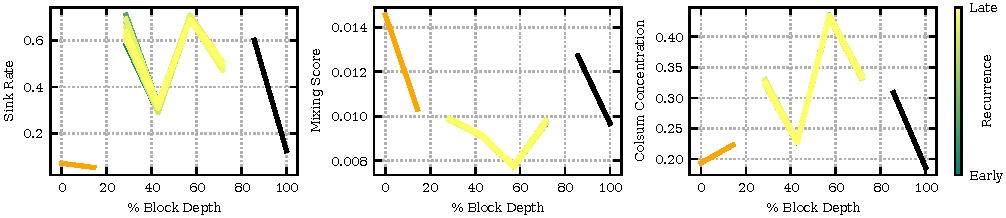
\includegraphics[width=\linewidth]{figures/orbits_sliders/huginn_stability_in_percentage_depth.pdf}
    \caption{Stages of inference metrics (sink rate, mixing score and colsum concentration) for \raven{} across 128 recurrences, for the GSM8k test prompt that exhibited the largest orbit amplitude: only the final 64 recurrences are visualized, to isolate the impact of the orbit. Visualized in percentage block depth.}
    \label{fig:orbits_sliders_huginn_stability_in_depth}
\end{figure}

We plot the same for the largest amplitude orbit on the \rllama{} model in \Cref{fig:orbits_sliders_llama_stability_in_depth}, demonstrating that the same behavior holds.

\begin{figure}[ht]
    \centering
    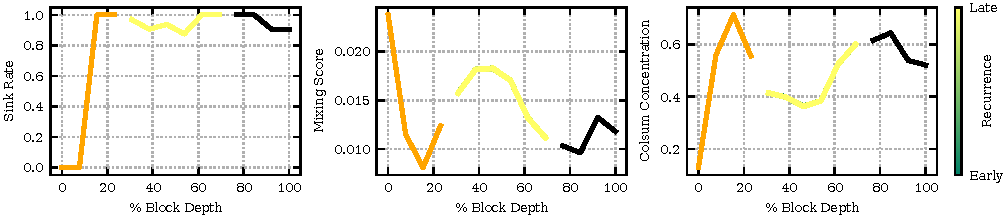
\includegraphics[width=\linewidth]{figures/orbits_sliders/stability_in_percentage_depth_llama.pdf}
    \caption{Stages of inference metrics (sink rate, mixing score and colsum concentration) for \rllama{} across 128 recurrences, for the GSM8k test prompt that exhibited the largest orbit amplitude: only the final 64 recurrences are visualized, to isolate the impact of the orbit. Visualized in percentage block depth.}
    \label{fig:orbits_sliders_llama_stability_in_depth}
\end{figure}

\FloatBarrier
\section{Additional Fixed Point Results}\label{appen:additional_fixed_point_results}
\FloatBarrier
\subsection{Cyclic Similarity}\label{appen:additional_cyclic_similarity}

We include here additional plots to validate our cyclic similarity claims in \Cref{sec:cyclic_similarity}.

\Cref{fig:similar_residual_stream_cosine} complements \Cref{fig:similar_attention_patterns} by visualizing the cosine similarity between the residual streams after each layer for the range of Looped Transformers visualized in the original figure. Additional models (\raven{} and all retrofitted models) are visualized in \Cref{fig:similar_residual_stream_cosine} for 32 recurrences, demonstrating that the cyclic similarity is consistent for larger numbers of recurrences. We note that \raven{} continues its previous trend of all layer outputs converging to similar representations, with some cyclic similarity still visible. \Cref{fig:similar_attention_patterns_expanded} similarly provides an extended version of \Cref{fig:similar_attention_patterns}, demonstrating that attention matrix cyclic similarity holds to 32 recurrences.

\begin{figure*}[ht]
    \centering
    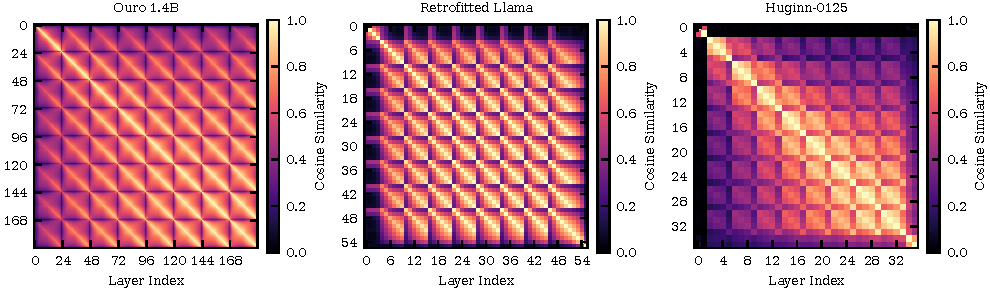
\includegraphics[width=0.9\linewidth]{figures/fixed_point/heatmaps/residual_stream_cosine_similarities.pdf}
    \vspace{-0.4cm}
    \caption{\textbf{Cosine similarity between residual streams after every pair of layers for different Transformer models}, averaged across the batch and sequence dimensions. \textbf{Left:} \ouro{} 1.4B \citep{zhu2025scaling}. \textbf{Center:} Retrofitted Llama \citep{mcleish2025teaching}. \textbf{Right:} \raven{} \citep{geiping2025scaling}. All models looped 8 times. Diagonal patterns indicate that the residual stream after each sub-block is most similar to the same block in the next recurrence; every layer in the recurrent block reaches a different fixed point.}
    \label{fig:similar_residual_stream_cosine}
\end{figure*}

\begin{figure}[ht]
    \centering
    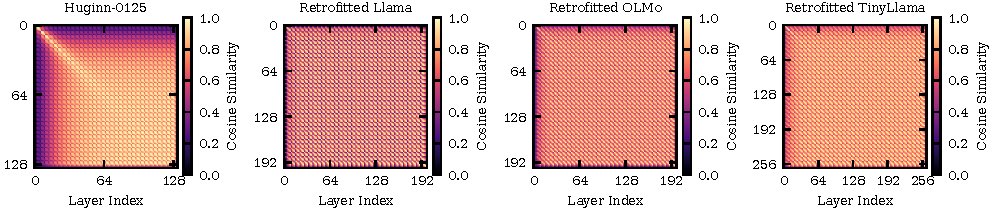
\includegraphics[width=\linewidth]{figures/fixed_point/heatmaps/residual_stream_cosine_similarities_expanded.pdf}
    \caption{Cosine similarity between residual streams after every pair of layers for different Transformer models, averaged across the batch and sequence dimensions. \textbf{Left:} \raven{} \citep{geiping2025scaling}. \textbf{Center Left:} Retrofitted Llama. \textbf{Center Right:} Retrofitted OLMo. \textbf{Right:} Retrofitted TinyLlama \citep{mcleish2025teaching}. All models looped 32 times. Extended version of \Cref{fig:similar_residual_stream_cosine}.}
    \label{fig:similar_residual_stream_cosine_expanded}
\end{figure}


\begin{figure}[ht]
    \centering
    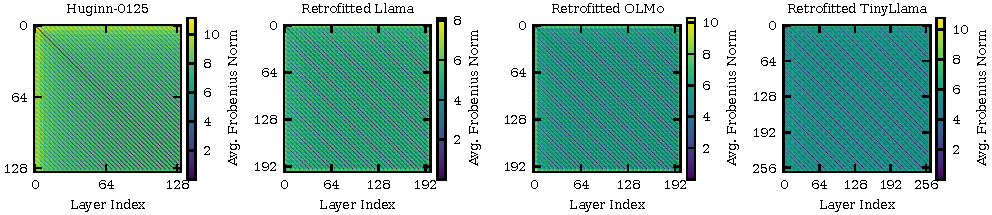
\includegraphics[width=\linewidth]{figures/fixed_point/heatmaps/attention_weight_norms_expanded.pdf}
    \caption{Frobenius norm between attention matrices for different Transformer models, averaged across the batch and head dimensions. \textbf{Left:} \raven{} \citep{geiping2025scaling}. \textbf{Center Left:} Retrofitted Llama. \textbf{Center Right:} Retrofitted OLMo. \textbf{Right:} Retrofitted TinyLlama \citep{mcleish2025teaching}. All models looped 32 times. Extended version of \Cref{fig:similar_attention_patterns}.}
    \label{fig:similar_attention_patterns_expanded}
\end{figure}

\FloatBarrier
\subsection{Fixed Point and Successive Differences}

In \Cref{sec:cyclic_similarity} we demonstrate that retrofitted Llama and \raven{} reach a fixed point but \ouro{} does not. We do so by -- for each layer -- computing an ``approximate fixed point'' after 128 recurrences and then plotting the norm of the difference for each layer at successive recurrences to this fixed point. In \Cref{fig:fixed_point_cosine_similarities} we demonstrate that this same behavior is observed when considering \emph{cosine similarity} to the fixed point, and in \Cref{fig:fixed_point_attention_differences} we see that it holds for attention matrices.

\begin{figure}[ht]
    \centering
    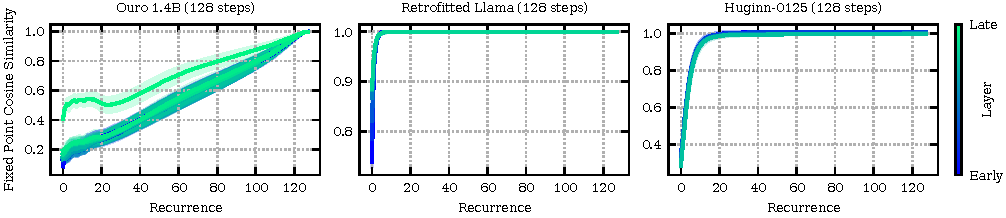
\includegraphics{figures/fixed_point/recurrencewise/fixed_point_cosine_similarities.pdf}
    \caption{\textbf{Cosine similarity between the residual stream after each layer in the recurrent block and its ``approximate fixed point''} - the residual stream after that layer in the 128th recursion. While \raven{} and retrofitted Llama quickly reach a fixed point, \ouro{} does not - even though the cosine similarity between successive recursions tends towards one, as evidenced by \Cref{fig:fixed_point_cosine_similarities}.}
    \label{fig:fixed_point_cosine_similarities}
\end{figure}

\begin{figure}[ht]
    \centering
    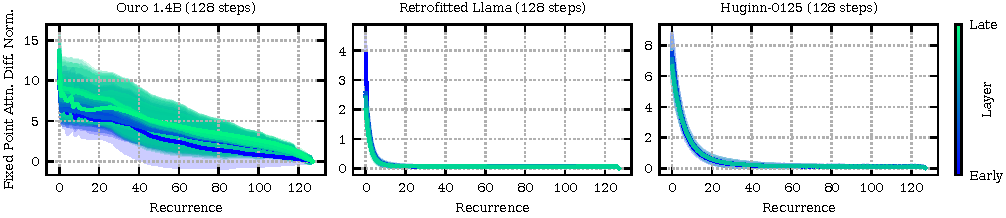
\includegraphics{figures/fixed_point/recurrencewise/fixed_point_attention_differences.pdf}
    \caption{\textbf{Frobenius norm between attention matrices of each layer in the recurrent block and their corresponding ``approximate fixed point''}; the attention matrices of the same layer in the 128th recursion. While \raven{} and retrofitted Llama quickly reach a fixed point, \ouro{} does not.}
    \label{fig:fixed_point_attention_differences}
\end{figure}

We then demonstrated in \Cref{fig:successive_norms} that all models, independent of whether they reach a strict fixed point or not, demonstrate converge towards very low difference norms between successive residual streams. We verify this same behavior holds for residual stream cosine similarities and attention matrix Frobenius norms in \Cref{fig:successive_cosine_similarities,fig:successive_attention_norms} respectively.

\begin{figure}[ht]
    \centering
    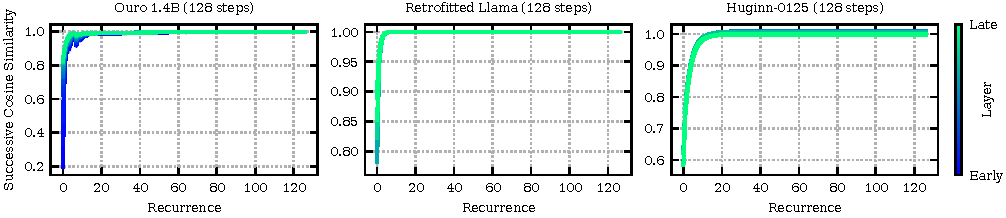
\includegraphics{figures/fixed_point/recurrencewise/successive_cosine_similarities.pdf}
    \caption{Cosine similarities between successive recursions of the residual stream after the same layer.}
    \label{fig:successive_cosine_similarities}
\end{figure}

\begin{figure}[ht]
    \centering
    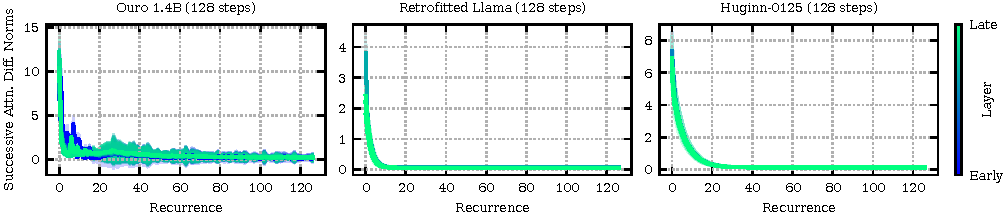
\includegraphics{figures/fixed_point/recurrencewise/successive_attention_differences.pdf}
    \caption{{Frobenius norm between attention matrices of each layer between successive recurrences.}}
    \label{fig:successive_attention_norms}
\end{figure}

\FloatBarrier
\subsection{Latent Space Trajectories}

In this section we visualize additional latent space trajectories, supplementing \Cref{fig:retro_llama_trajectory}. All trajectories are plotted by taking all latent states of the final token position on the test sequence described in \Cref{appen:experiment_details}, computing PCA on these latent state vectors and resultant dimensional reduction of this sequence of vectors. They are intended as illustrations to demonstrate qualitative behavior. \ouro{} is visualized in \Cref{fig:ouro_trajectory} and \raven{} in \Cref{fig:raven_trajectory}.

The \ouro{} trajectory is of particular interest as we are aware from the results in the main body of the paper that this model does not reach a strict fixed point. \Cref{fig:ouro_trajectory} demonstrates that -- on this test sequence -- \ouro{} reaches an approximately constant trajectory, but with visibly larger deviations even at later recurrences than \raven{} in \Cref{fig:raven_trajectory}.

However, we find evidence that this ``approximately stable trajectory'' behavior is not universal: for a simple ``maths'' test prompt (\texttt{The square root of 16 is}) shown in \Cref{fig:ouro_maths_trajectory}, \ouro{} appears to reach a stable trajectory in recurrences 8-16 before departing from this and appearing to become ``unstable''.

\begin{figure}[ht]
    \centering
    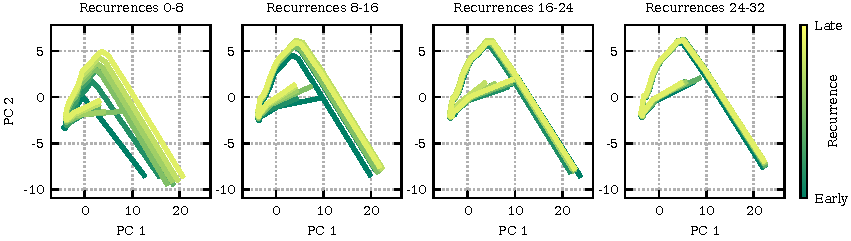
\includegraphics{figures/trajectory/pca_quartiles_Ouro_1.4B_32_steps_extended.pdf}
    \caption{\textbf{\ouro{} 1.4B \citep{zhu2025scaling} latent space trajectory} traced out by the hidden states of the final sequence position on the test prompt; reduced to two dimensions by computing PCA over all final sequence position embeddings.}
    \label{fig:ouro_trajectory}
\end{figure}

\begin{figure}[ht]
    \centering
    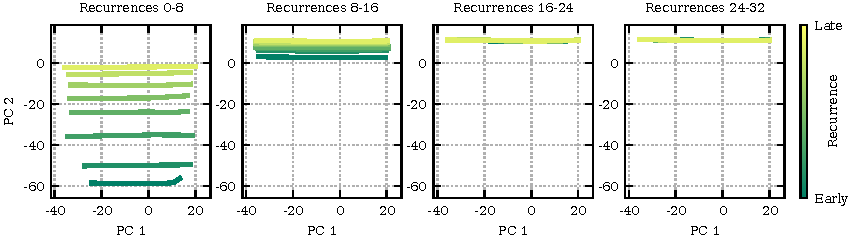
\includegraphics{figures/trajectory/pca_quartiles_Huginn-0125_32_steps_extended.pdf}
    \caption{\textbf{\raven{} \citep{geiping2025scaling} latent space trajectory} traced out by the hidden states of the final sequence position on the test prompt; reduced to two dimensions by computing PCA over all final sequence position embeddings.}
    \label{fig:raven_trajectory}
\end{figure}

\begin{figure}[ht]
    \centering
    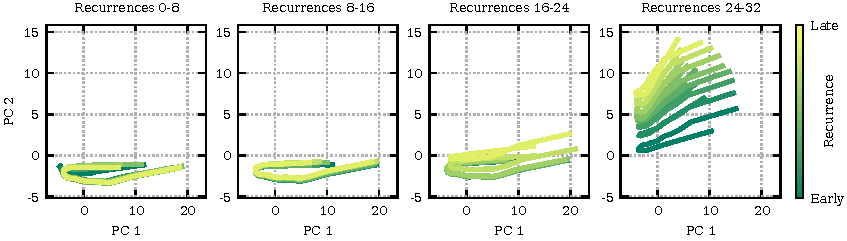
\includegraphics{figures/trajectory/maths_pca_quartiles_Ouro_1.4B_32_steps_extended.pdf}
    \caption{\textbf{\ouro{} 1.4B \citep{zhu2025scaling} latent space trajectory} traced out by the hidden states of the final sequence position on a ``maths'' test prompt (\texttt{The square root of 16 is}); reduced to two dimensions by computing PCA over all final sequence position embeddings.}
    \label{fig:ouro_maths_trajectory}
\end{figure}

\FloatBarrier
\subsection{Architecture Choices}

Here we provide more complete results to supplement \Cref{subsec:norm_and_ii}, visualizing fixed point difference norms and cosine similarities for various architecture choices in \Cref{fig:stability_initialised_fixed_point_norms,fig:stability_initialised_fixed_point_cosine_similarities} respectively.

\begin{figure}[ht]
    \centering
    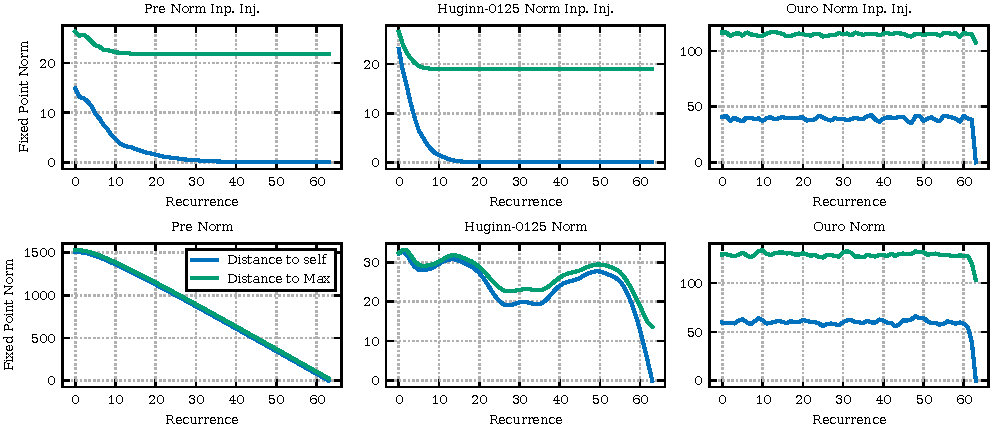
\includegraphics[width=0.8\linewidth]{figures/fixed_point/stability_initialised_fixed_point_norms.pdf}
    \caption{\textbf{Norm of the difference between the residual stream after the first layer in the recurrent block for successive recurrences and an ``approximate fixed point''} -- the residual stream in the 128th recurrence. Two fixed point differences are visualized: the difference to the fixed point of the same (first) layer (blue) and the difference to the fixed point which has the greatest norm difference from the first layer (green). Visualized are a range of norm structures (columns), with input injection (top row) and without (bottom row). All models are randomly initialized with 12 layers in the recurrent block, and no prelude or coda.}
    \label{fig:stability_initialised_fixed_point_norms}
\end{figure}

\begin{figure}[ht]
    \centering
    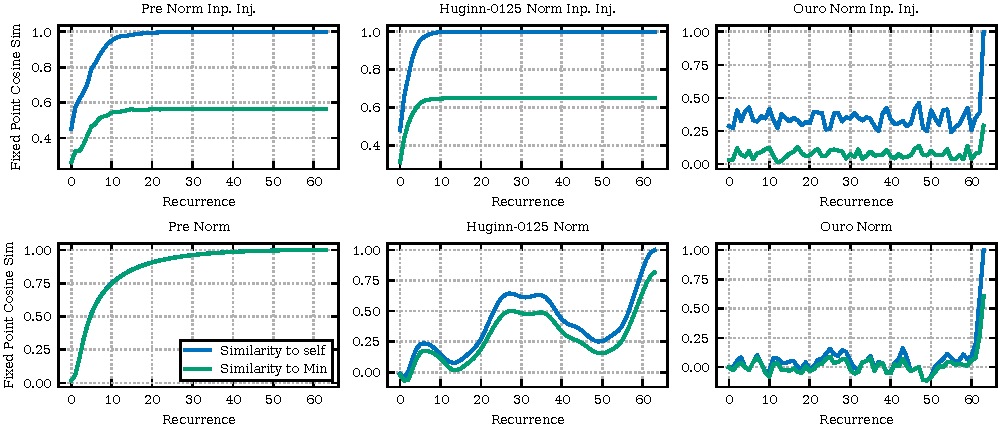
\includegraphics[width=0.8\linewidth]{figures/fixed_point/stability_initialised_fixed_point_cosine_similarities.pdf}
    \caption{\textbf{Cosine similarity between the residual stream after the first layer in the recurrent block for successive recurrences and an ``approximate fixed point''} -- the residual stream in the 128th recurrence. Two fixed point differences are visualized: the difference to the fixed point of the same (first) layer (blue) and the difference to the fixed point which has the lowest cosine similarity to the first layer (green). Visualized are a range of norm structures (columns), with input injection (top row) and without (bottom row). All models are randomly initialized with 12 layers in the recurrent block, and no prelude or coda.}
    \label{fig:stability_initialised_fixed_point_cosine_similarities}
\end{figure}

We also verify that the results presented are not particular to 12 layers by visualising results for both 4 and 16 layers in \Cref{fig:stability_initialised_fixed_point_cosine_similarities_multiple_layers}, showing qualitatively identical behavior.

\begin{figure}[ht]
    \centering
    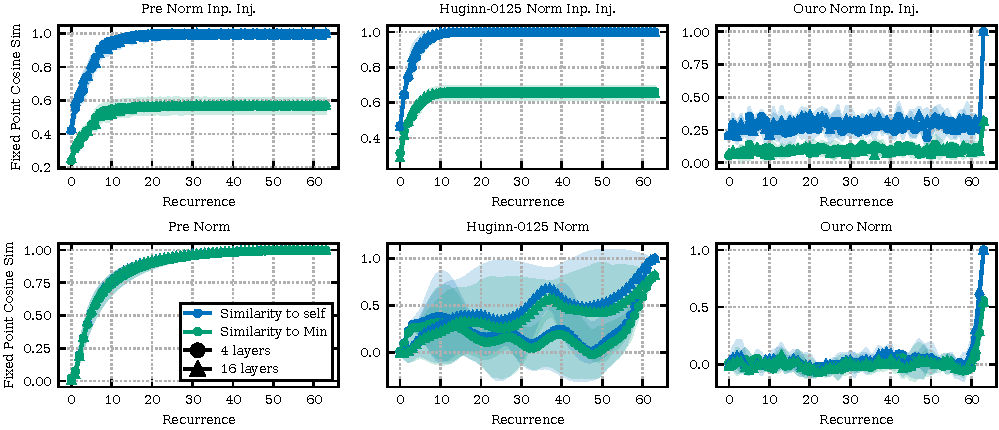
\includegraphics[width=0.8\linewidth]{figures/fixed_point/stability_initialised_final_state_difference_sim_multiple_layers.pdf}
    \caption{\textbf{Cosine similarity between the residual stream after the first layer in the recurrent block for successive recurrences and an ``approximate fixed point''} -- the residual stream in the 128th recurrence. Two fixed point differences are visualized: the difference to the fixed point of the same (first) layer (blue) and the difference to the fixed point which has the lowest cosine similarity to the first layer (green). Visualized are a range of norm structures (columns), with input injection (top row) and without (bottom row). Here models of 4 and 16 layers are compared, showing qualitatively identical behavior and demonstrating that the behavior is not particular to 12 layers.}
    \label{fig:stability_initialised_fixed_point_cosine_similarities_multiple_layers}
\end{figure}

\FloatBarrier
\section{Additional Stages of Inference Results}\label{appen:additional_soi_results}

In this appendix we explore in more detail the mixing behavior presented in the main body via additional metrics, and considering a wider range of models.

\subsection{Input Independent Metrics}

As our work is concerned largely with how the functionality of layers change throughout depth as the residual stream is iteratively updated, our primary concern is with \emph{input-dependent} measures of stages of inference: ColSum concentration as presented in the main text of the paper is one such input-dependent metric, and the later sections of this appendix will introduce and present results for a wider range of such metrics.

However, to bridge the gap between our work and that of \citet{lad2024remarkable}, we also present results for the fraction of \emph{prediction and suppression} neurons \citep{gurnee2024universal} in successive layers of both feedforward and looped Transformers. We highlight however that \emph{these are unable to change with successive recurrences}, and are thus secondary to our focus. \Cref{fig:feedforward_prediction_neurons} presents results for a selection of feedforward models used throughout the paper, and \Cref{fig:looped_prediction_neurons} presents results for a selection of looped models used throughout the paper. Similar to our results elsewhere, we find that the looped model stages of inference in these metrics tend to mirror those of feedforward models.

\begin{figure*}[ht]
    \centering    
    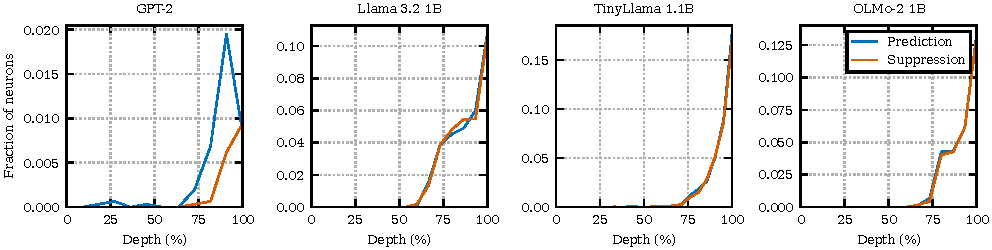
\includegraphics{figures/prediction_neurons/feedforward.pdf}
    \caption{\textbf{Fraction of prediction and suppression neurons in a selection of feedforward models used throughout the paper}.}
    \label{fig:feedforward_prediction_neurons}
\end{figure*}

\begin{figure*}[ht]
    \centering    
    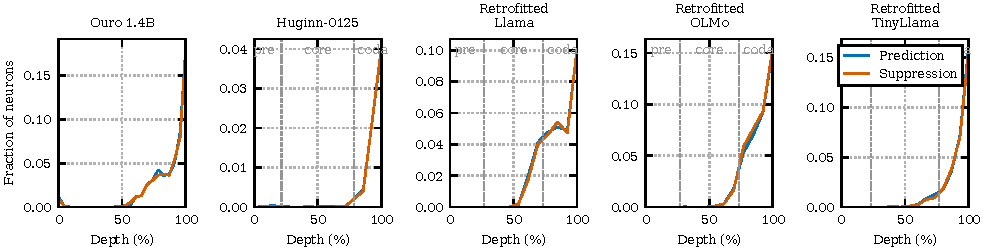
\includegraphics{figures/prediction_neurons/looped.pdf}
    \caption{\textbf{Fraction of prediction and suppression neurons in a selection of looped models used throughout the paper}.}
    \label{fig:looped_prediction_neurons}
\end{figure*}

\subsection{Input Dependent Metrics}\label{appen:input_dependent_soi_metrics}

One well-studied phenomenon by which Transformers drastically \emph{reduce} the mixing in given layer is that of the \emph{attention sink} \citep{xiao2023efficient,barbero2025llms}, whereby the layer focuses the majority of the attention ``weight'' onto the first token in the sequence; often this is the BOS (beginning of sequence) token, and thus completely uninformative. To measure this behavior, we adopt the \textbf{attention sink score} and \textbf{sink rate} of \citet{gu2024attention}: for token position $k$ and sequence length $T$, the sink score at layer $\ell$ and head $h$ is defined as:
\begin{equation}
    \text{sink-score}_k^{(\ell,h)} = \frac{1}{T}\sum_{t=0}^{T-1}A_{tk}^{(\ell,h)},
\end{equation}
where $A_{tk}^{(\ell,h)}$ corresponds to the realized attention matrix of \Cref{eq:attn_in_a} at layer $\ell$, head $h$. The sink rate is then defined as the fraction of heads for which the sink score lies above a certain threshold:
\begin{equation}
    \text{sink-rate}^{(\ell)}_k = \frac{1}{H}\sum_{h=1}^H\mathbb{I}\!\left(\text{sink-score}_k^{(\ell,h)}\geq \tau\right),
\end{equation}
where following related work we define a threshold of $\tau=0.3$, and $\mathbb{I}$ denotes the indicator function.

We also adopt the \emph{Mixing score} of \citet{queipo2025attention}: for sequence length $T$, layer $\ell$ and head $h$ this is defined as the average row entropy of the attention matrices:
\begin{equation}
    \text{mixing-score}^{(\ell,h)} = \frac{1}{T} \sum_{i=1}^T H(A_{i, :}^{(\ell, h)}).
\end{equation}

Following \citet{skean2025layer,queipo2025attention} we additionally measure the compression of the residual stream $\mX$ via the matrix-based entropy $H(\mX)$.

In the plots that follow we average sink rates, Mixing scores and ColSum concentrations over all the heads in a layer, and over all input sequences. Residual entropy is averaged over all input sequences.

\FloatBarrier
\subsection{Cyclic Stages of Inference}\label{appen:cyclic_soi}

Supplementing the cyclic recurrence in realized depth for retrofitted Llama in \Cref{fig:stages_of_inference_cyclic_and_similar}, we additionally overlay cycles in realized depth for \ouro{} and \raven{} in \Cref{fig:stages_of_inference_cyclic_extended}, where all models are run for 8 recurrences. This demonstrates that for \textbf{sink rates and mixing scores}, the cyclic behavior and lack of significant depth-wise changes hold both for the other investigated models, and the additional stages of inference metrics.

The results for residual entropy are more nuanced: while the results for \raven{} and the retrofitted models show broadly the same behavior as the attention-based metrics, \ouro{} demonstrates different behavior. As shown in \Cref{fig:ouro_recurrent_block_stages}, the residual entropies both change significantly with successive recurrences and do not closely follow the feedforward behavior. We believe that the divergence from feedforward behavior may derive from the norm structure of this model: the residual stream is normalised after each recurrent block, as visualised in \Cref{fig:residual_norm_comparison}, thus periodically shutting down massive activations. This is not the case for the retrofitted series of models, which lack this norm and show much closer alignment with feedforward stages of inference.

\begin{figure*}[ht]
    \centering    
    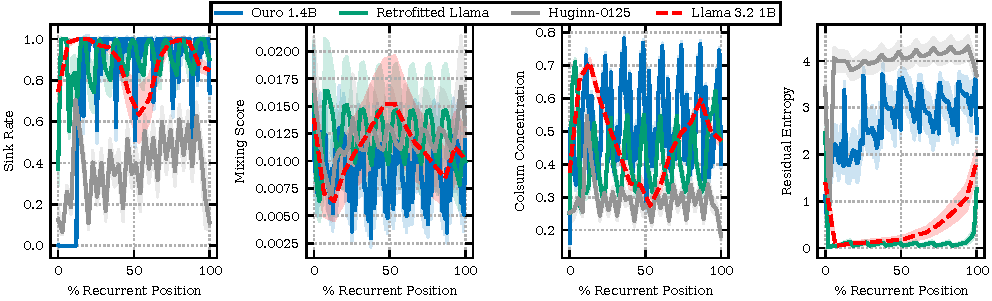
\includegraphics{figures/stages_of_inference/cyclic_behaviour_extended.pdf}
    \caption{\textbf{Stages of inference for a selection of Looped transformers, all using 8 recurrences}: \raven{} \citep{geiping2025scaling}, Ouro 1.4B \citep{zhu2025scaling} and Llama with retrofitted recurrences \citep{mcleish2025teaching}. Note \raven{} and Retrofitted Llama have prelude and coda layers too: each 2 layers in \raven{} and each 4 in Retrofitted Llama.}
    \label{fig:stages_of_inference_cyclic_extended}
\end{figure*}

For completeness, we plot these stages of inference for all other models referenced in the paper. See \Cref{fig:ouro_recurrent_block_stages} (Ouro 1.4B), \Cref{fig:raven_recurrent_block_stages} (\raven{}), \Cref{fig:retrofitted_llama_recurrent_block_stages,fig:retrofitted_olmo_recurrent_block_stages,fig:retrofitted_tinyllama_recurrent_block_stages} (retrofitted Llama, OLMo and TinyLlama).

\begin{figure}
    \centering    
    
\includegraphics{figures/stages_of_inference/recurrent/Ouro_1.4B_4_steps.pdf}
    \caption{\textbf{Stages of inference for each recurrent loop in Ouro 1.4B.} The close overlap with feedforward stages of inference is a particularly striking result as this model is trained from scratch with recurrence.}
    \label{fig:ouro_recurrent_block_stages}
\end{figure}

\begin{figure}
    \centering    
    
\includegraphics{figures/stages_of_inference/recurrent/Huginn-0125.pdf}
    \caption{\textbf{Stages of inference for each recurrent loop in \raven{}.} This represents a negative result: stages of inference do not occur. We discuss possible causes for this in the main text.}
    \label{fig:raven_recurrent_block_stages}
\end{figure}

\begin{figure}
    \centering    
    
\includegraphics{figures/stages_of_inference/recurrent/Retrofitted_Llama.pdf}
    \caption{\textbf{Stages of inference for each recurrent loop in the retrofitted Llama model \citep{mcleish2025teaching}.} Each block demonstrates very similar stages of inference to Llama, the base model from which pretrained layers are taken.}
    \label{fig:retrofitted_llama_recurrent_block_stages}
\end{figure}

\begin{figure}
    \centering    
    
\includegraphics{figures/stages_of_inference/recurrent/Retrofitted_OLMo.pdf}
    \caption{\textbf{Stages of inference for each recurrent loop in the retrofitted OLMo model \citep{mcleish2025teaching}.} Similarly, each block demonstrates very similar stages of inference to OLMo, the base model from which pretrained layers are taken.}
    \label{fig:retrofitted_olmo_recurrent_block_stages}
\end{figure}

\begin{figure}
    \centering    
    
\includegraphics{figures/stages_of_inference/recurrent/Retrofitted_TinyLlama.pdf}
    \caption{\textbf{Stages of inference for each recurrent loop in the retrofitted TinyLlama model \citep{mcleish2025teaching}.} Similarly, each block demonstrates very similar stages of inference to TinyLlama, the base model from which pretrained layers are taken.}
    \label{fig:retrofitted_tinyllama_recurrent_block_stages}
\end{figure}

We plot stages of inference for \ouro{} 2.6B in \Cref{fig:ouro_2_recurrent_block_stages}. This model is interesting due to the training regime followed by \citet{zhu2025scaling}, which ``upcycles'' a 48 layer model from the 24 layer 1.4B parameter model. As a consequence, the first and second half of each recurrent block each independently align with the Llama feedforward stages of inference.

\begin{figure}
    \centering    
    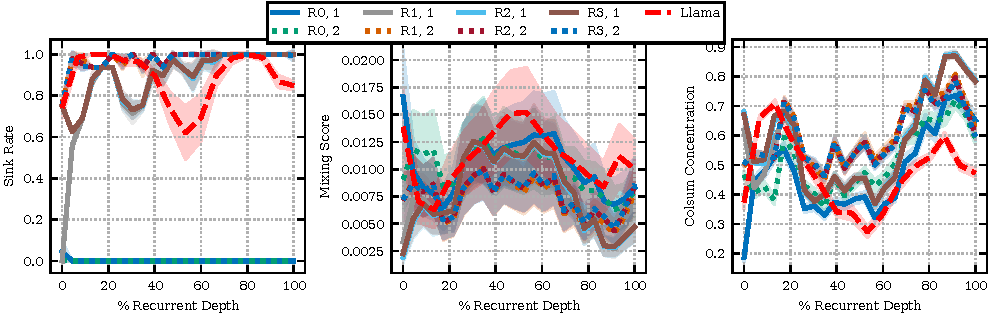
\includegraphics{figures/stages_of_inference/recurrent/Ouro_2.6B.pdf}
    \caption{\textbf{Stages of inference for each recurrent loop in Ouro 2.6B.} For this model we separate out the first and second half of the recurrent block and overlay them, demonstrating that both halves have close alignment with the Llama feedforward stages of inference. We suggest that this likely arises due to the training regime of \citet{zhu2025scaling}, which first trains a single 24 layer 1.4B parameter model, and then ``upcycles'' this into a 48 layer 2.6B parameter model by duplicating these layers, consequently duplicating the stages of inference as well.}
    \label{fig:ouro_2_recurrent_block_stages}
\end{figure}

In \Cref{sec:stages_of_inference} we suggested that the lack of stages of inference in \raven{} is likely due to the normalization of the residual stream resulting in massive activations being unable to form. Here we further support this suggestion by ablating the massive activations from the \rllama{} model (which \emph{does} display stages of inference) via zeroing the output of the MLP in the second layer, which is responsible for its massive activations. In this setting, visualized in \Cref{fig:ablation_rllama}, we see that the model no longer exhibits stages of inference comparable to the feedforward model, suggesting that the presence of massive activations is required for stages of inference to emerge in looped models.

\begin{figure}
    \centering    
    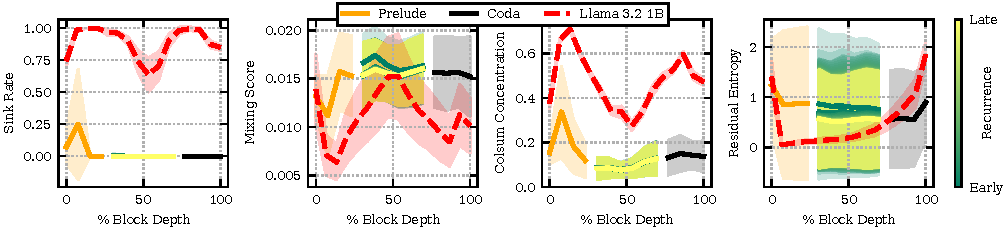
\includegraphics{figures/stages_of_inference/ablation_retrofitted_llama_bos_mlp.pdf}
    \caption{\textbf{Stages of inference for each recurrent loop in \rllama{} for which the massive activations have been ablated.} }
    \label{fig:ablation_rllama}
\end{figure}

\FloatBarrier
\subsection{Non-Reasoning Stages of Inference}\label{appen:hellaswag_soi}

Throughout the rest of the paper, experiments are conducted on the GSM8k dataset. In this appendix we verify that the stages of inference we observe are not specific to this dataset, and also occur in a non-reasoning setting, for which we use the HellaSwag dataset \citep{zellers2019hellaswag}. We follow an identical experimental setup to the GSM8k experiments, running inference on 256 random examples from the test split.

We present results in \Cref{fig:ouro_recurrent_block_stages_hellaswag} (Ouro 1.4B), \Cref{fig:raven_recurrent_block_stages_hellaswag} (\raven{}), \Cref{fig:retrofitted_llama_recurrent_block_stages_hellaswag,fig:retrofitted_olmo_recurrent_block_stages_hellaswag,fig:retrofitted_tinyllama_recurrent_block_stages_hellaswag} (retrofitted Llama, OLMo and TinyLlama). These show very few deviations from the GSM8k results, and the conclusions throughout the rest of the paper hold. However, we highlight the following small differences:
\begin{itemize}
    \item Across the board, sink rates tend to be higher in the HellaSwag setting.
    \item In \rolmo{}, ColSum concentration appears to be slightly higher in the HellaSwag setting.
\end{itemize}


\begin{figure}[ht]
    \centering    
    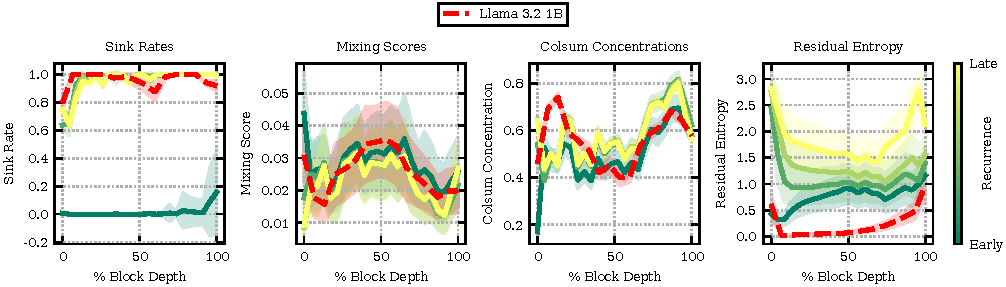
\includegraphics{figures/hellaswag/stages_of_inference/recurrent/Ouro_1.4B_4_steps.pdf}
    \caption{\textbf{Stages of inference for each recurrent loop in Ouro 1.4B, run on the HellaSwag dataset.}}
    \label{fig:ouro_recurrent_block_stages_hellaswag}
\end{figure}

\begin{figure}[ht]
    \centering    
    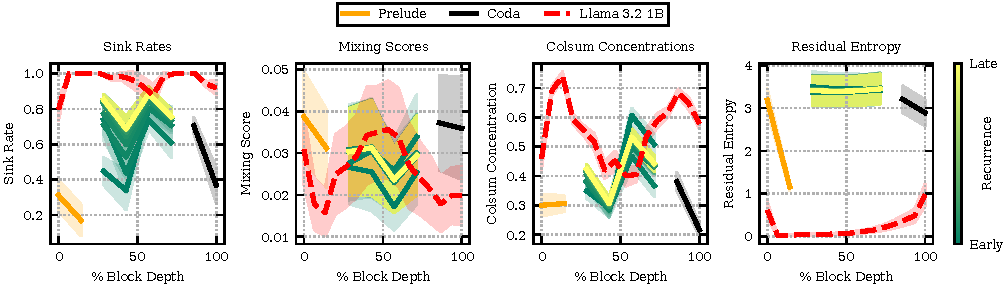
\includegraphics{figures/hellaswag/stages_of_inference/recurrent/Huginn-0125.pdf}
    \caption{\textbf{Stages of inference for each recurrent loop in \raven{}, run on the HellaSwag dataset.}}
    \label{fig:raven_recurrent_block_stages_hellaswag}
\end{figure}

\begin{figure}[ht]
    \centering    
    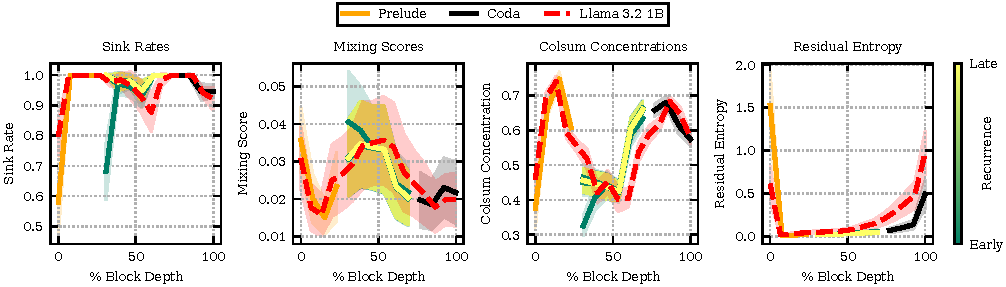
\includegraphics{figures/hellaswag/stages_of_inference/recurrent/Retrofitted_Llama.pdf}
    \caption{\textbf{Stages of inference for each recurrent loop in the retrofitted Llama model \citep{mcleish2025teaching}, run on the HellaSwag dataset.}}
    \label{fig:retrofitted_llama_recurrent_block_stages_hellaswag}
\end{figure}

\begin{figure}[ht]
    \centering    
    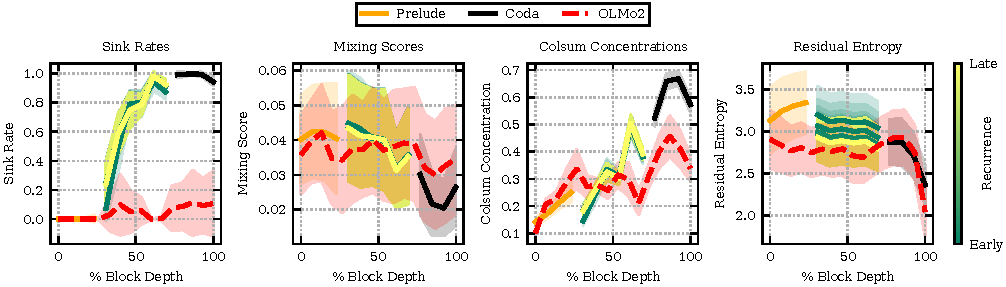
\includegraphics{figures/hellaswag/stages_of_inference/recurrent/Retrofitted_OLMo.pdf}
    \caption{\textbf{Stages of inference for each recurrent loop in the retrofitted OLMo model \citep{mcleish2025teaching}, run on the HellaSwag dataset.} ColSum concentration deviates slightly from its GSM8k counterpart here, but still broadly follows the same stages of inference as the feedforward OLMo model.}
    \label{fig:retrofitted_olmo_recurrent_block_stages_hellaswag}
\end{figure}

\begin{figure}[ht]
    \centering    
    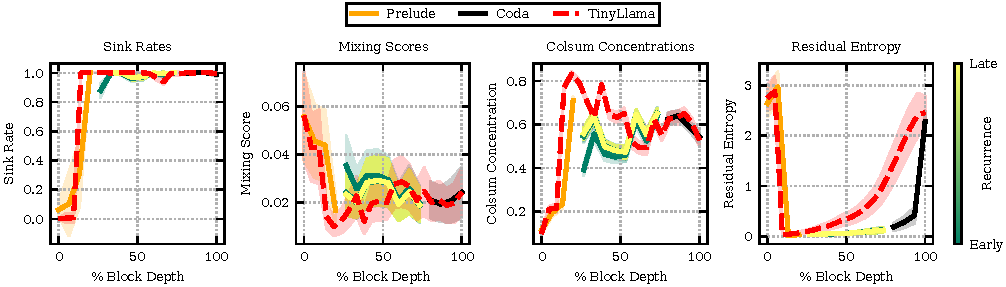
\includegraphics{figures/hellaswag/stages_of_inference/recurrent/Retrofitted_TinyLlama.pdf}
    \caption{\textbf{Stages of inference for each recurrent loop in the retrofitted TinyLlama model \citep{mcleish2025teaching}, run on the HellaSwag dataset.}}
    \label{fig:retrofitted_tinyllama_recurrent_block_stages_hellaswag}
\end{figure}

\FloatBarrier
\subsection{Stability To Unseen Test-Time Recurrences}

This section extends the results presented in \Cref{sec:stability}.

We supplement \Cref{fig:stability_in_total_recurrence} by plotting how stages of inference change per-layer throughout recurrences for additional models: these can be found in \Cref{fig:stages_of_inference_ouro_stability,fig:stages_of_inference_raven_stability,fig:stages_of_inference_retro_llama_stability}. The large standard deviations in \raven{} and retrofitted Llama mixing scores reflect the fact that these models tend to reach different, but still stable, constant states.

\begin{figure}[ht]
    \centering    
    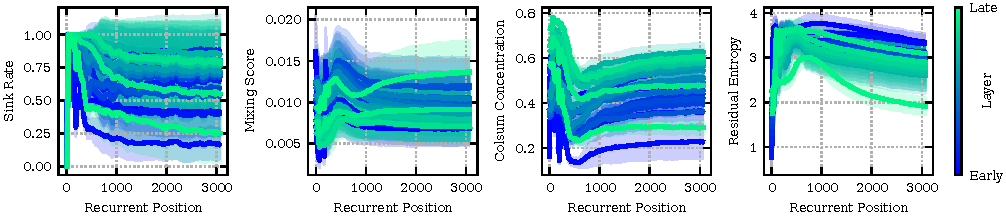
\includegraphics{figures/stages_of_inference/similar_behaviour/Ouro_1.4B_128_steps_means.pdf}
    \caption{\textbf{Stages of inference for each of the distinct blocks in \ouro{} \citep{zhu2025scaling}}, as they are reapplied throughout the model for 128 recurrences. These consistently change throughout the realized depth of the model, reaching no clear fixed point. Mean and standard deviation are over separate inputs to the model, taken over the GSM8k subset.}
    \label{fig:stages_of_inference_ouro_stability}
\end{figure}

\begin{figure}[ht]
    \centering    
    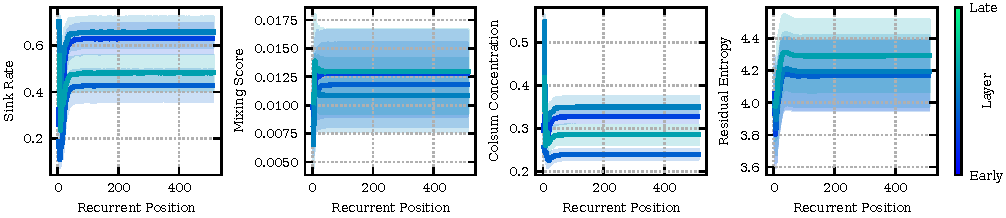
\includegraphics{figures/stages_of_inference/similar_behaviour/Huginn-0125_128_steps_means.pdf}
    \caption{\textbf{Stages of inference for each of the distinct blocks in \raven{} \citep{geiping2025scaling}}, as they are reapplied throughout the model for 128 recurrences. These converge to constant behavior. Mean and standard deviation are over separate inputs to the model, taken over the GSM8k subset.}
    \label{fig:stages_of_inference_raven_stability}
\end{figure}

\begin{figure}[ht]
    \centering    
    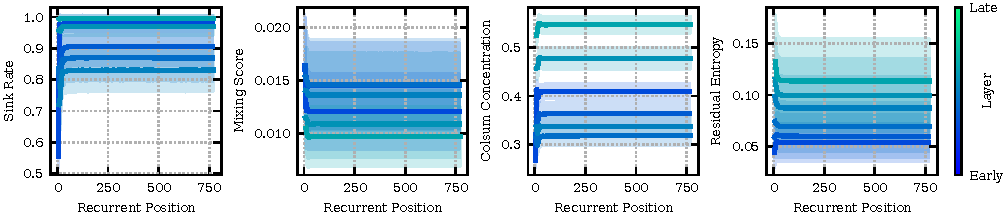
\includegraphics{figures/stages_of_inference/similar_behaviour/Retrofitted_Llama_128_steps_means.pdf}
    \caption{\textbf{Stages of inference for each of the distinct blocks in retrofitted Llama \citep{mcleish2025teaching},} as they are reapplied throughout the model for 128 recurrences. These converge to constant behavior. Mean and standard deviation are over separate inputs to the model, taken over the GSM8k subset.}
    \label{fig:stages_of_inference_retro_llama_stability}
\end{figure}

We additionally plot the extended versions of \Cref{fig:stability_in_percentage_depth} in \Cref{fig:stages_of_inference_ouro_stability_recurrence,fig:stages_of_inference_raven_stability_recurrence,fig:stages_of_inference_retro_llama_stability_recurrence}.

\begin{figure}[ht]
    \centering    
    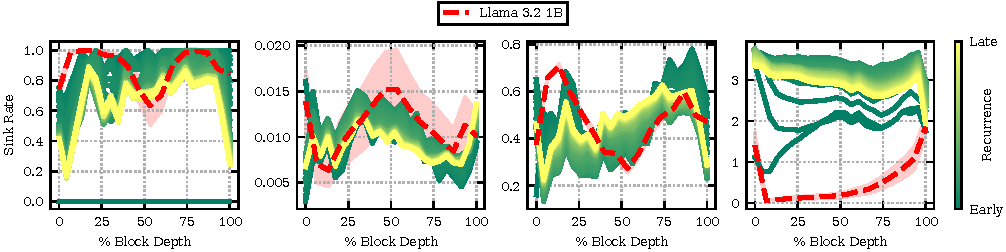
\includegraphics{figures/stages_of_inference/recurrent/Ouro_1.4B_128_steps_to_fixed_point.pdf}
    \caption{\textbf{Stages of inference for \ouro{} with each of 128 recurrences}, visualized over percentage recurrent depth. These consistently change with successive recurrences, deviating significantly from the stages of inference seen with train-time recurrences.}
    \label{fig:stages_of_inference_ouro_stability_recurrence}
\end{figure}

\begin{figure}[ht]
    \centering    
    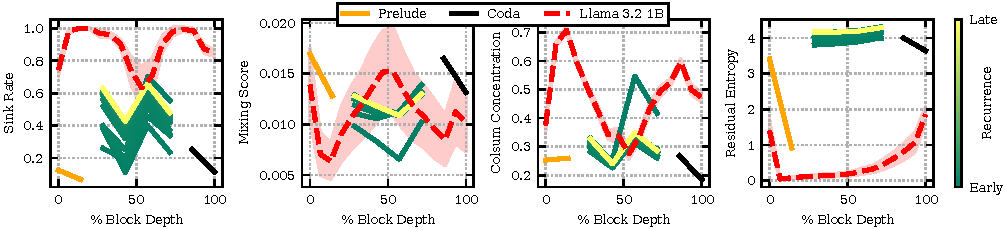
\includegraphics{figures/stages_of_inference/recurrent/Huginn-0125_128_steps_to_fixed_point.pdf}
    \caption{\textbf{Stages of inference for \raven{} with each of 128 recurrences}, visualized over percentage recurrent depth. These quickly reach a fixed point and do not deviate far from their starting stages of inference.}
    \label{fig:stages_of_inference_raven_stability_recurrence}
\end{figure}

\begin{figure}[ht]
    \centering    
    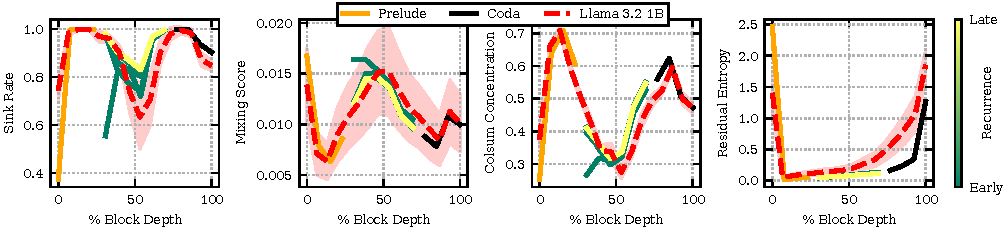
\includegraphics{figures/stages_of_inference/recurrent/Retrofitted_Llama_128_steps_to_fixed_point.pdf}
    \caption{\textbf{Stages of inference for retrofitted Llama with each of 128 recurrences}, visualized over percentage recurrent depth. These quickly reach a fixed point and do not deviate far from their starting stages of inference.}
    \label{fig:stages_of_inference_retro_llama_stability_recurrence}
\end{figure}

\begin{figure}[ht]
    \centering    
    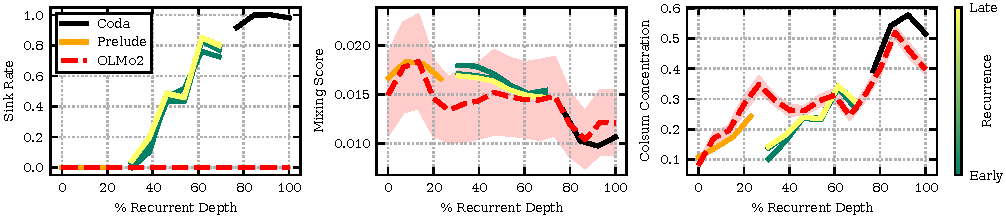
\includegraphics{figures/stages_of_inference/recurrent/Retrofitted_OLMo_128_steps_to_fixed_point.pdf}
    \caption{\textbf{Stages of inference for retrofitted OLMo-2 with each of 128 recurrences}, visualized over percentage recurrent depth. These quickly reach a fixed point and do not deviate far from their starting stages of inference.}
    \label{fig:stages_of_inference_retro_olmo_stability_recurrence}
\end{figure}

\FloatBarrier
\subsection{How Architecture Choices Affect the Formation of Stages of Inference}\label{appen:architecture_stages_of_inference}

Here we present additional results to supplement those in \Cref{sec:self_organising_soi}. The extended stages of inference metrics for the models visualized in \Cref{fig:summary_training_stages_of_interest} are presented in \Cref{fig:r4s,fig:r8s,fig:r12s}. Equivalent models with added input injection are visualized in \Cref{fig:r4si,fig:r8si,fig:r12si}, and equivalent models without sandwich layers in \Cref{fig:r4,fig:r8,fig:r12}.

It appears in these small scale experiments that feedforward stages of inference are most closely replicated without input injection, and using sandwich layers, as in \Cref{fig:r4s,fig:r8s,fig:r12s}. The addition of input injection appears to mean that the \emph{final} recurrence follows the feedforward stages of inference more closely, but to the detriment of earlier recurrences.

\begin{figure}[ht]
    \centering
    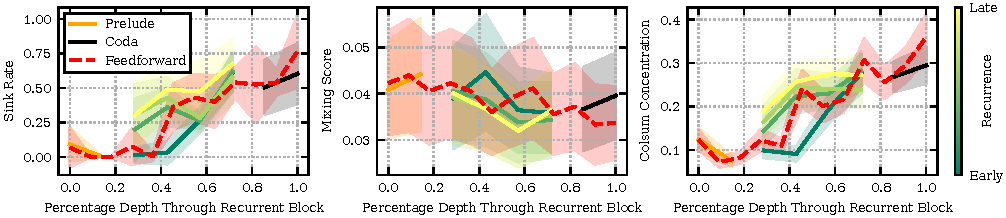
\includegraphics{figures/training/R4S.pdf}
    \caption{\textbf{Stages of inference metrics for a small-scale Looped Transformer of configuration $(2,4 \otimes 4,2)$}, compared to a ``control'' feedforward Transformer with the same training configuration and depth 12.}
    \label{fig:r4s}
\end{figure}

\begin{figure}[ht]
    \centering
    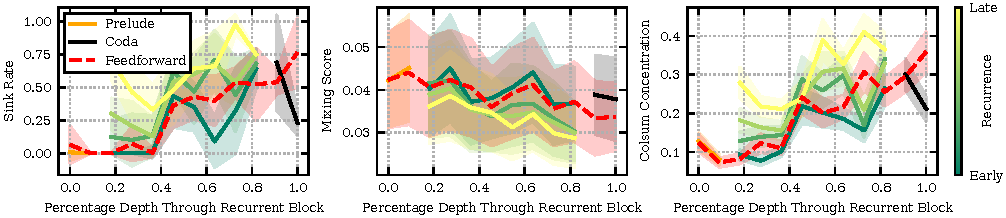
\includegraphics{figures/training/R8S.pdf}
    \caption{\textbf{Stages of inference metrics for a small-scale Looped Transformer of configuration $(2,8 \otimes 4,2)$}, compared to a ``control'' feedforward Transformer with the same training configuration and depth 12.}
    \label{fig:r8s}
\end{figure}

\begin{figure}[ht]
    \centering
    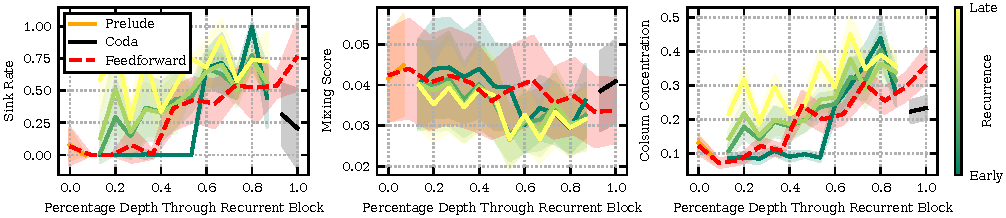
\includegraphics{figures/training/R12S.pdf}
    \caption{\textbf{Stages of inference metrics for a small-scale Looped Transformer of configuration $(2,12 \otimes 4,2)$}, compared to a ``control'' feedforward Transformer with the same training configuration and depth 12.}
    \label{fig:r12s}
\end{figure}

%%%%%%%%

\begin{figure}[ht]
    \centering
    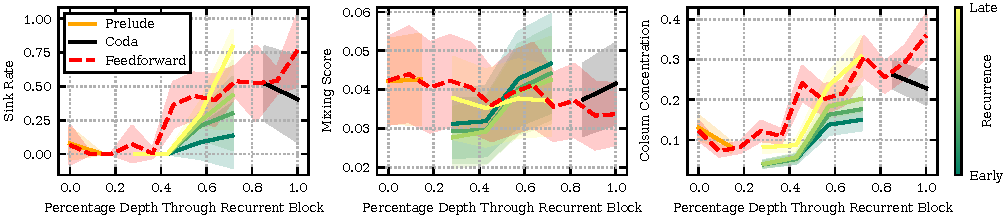
\includegraphics{figures/training/R4SI.pdf}
    \caption{\textbf{Stages of inference metrics for a small-scale Looped Transformer of configuration $(2,4 \otimes 4,2)_I$}, compared to a ``control'' feedforward Transformer with the same training configuration and depth 12.}
    \label{fig:r4si}
\end{figure}

\begin{figure}[ht]
    \centering
    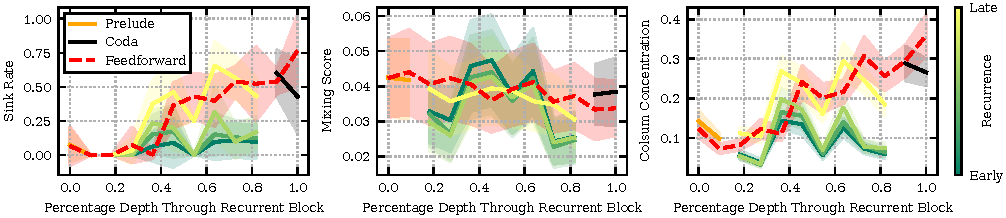
\includegraphics{figures/training/R8SI.pdf}
    \caption{\textbf{Stages of inference metrics for a small-scale Looped Transformer of configuration $(2,8 \otimes 4,2)_I$}, compared to a ``control'' feedforward Transformer with the same training configuration and depth 12.}
    \label{fig:r8si}
\end{figure}

\begin{figure}[ht]
    \centering
    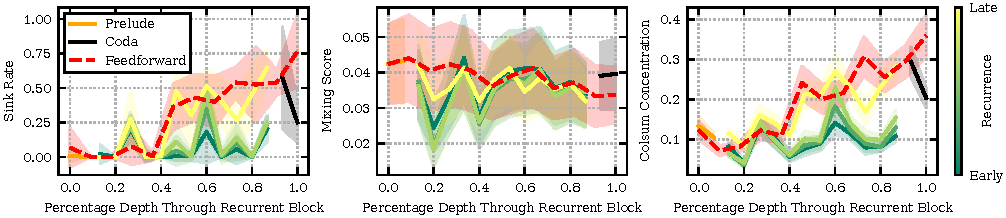
\includegraphics{figures/training/R12SI.pdf}
    \caption{\textbf{Stages of inference metrics for a small-scale Looped Transformer of configuration $(2,12 \otimes 4,2)_I$}, compared to a ``control'' feedforward Transformer with the same training configuration and depth 12.}
    \label{fig:r12si}
\end{figure}

%%%%%%

\begin{figure}[ht]
    \centering
    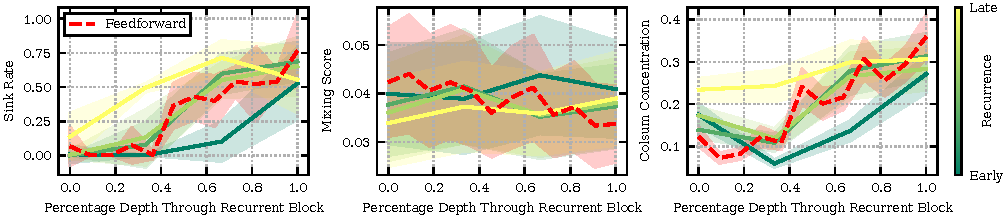
\includegraphics{figures/training/R4.pdf}
    \caption{\textbf{Stages of inference metrics for a small-scale Looped Transformer of configuration $(0,4 \otimes 4,0)$}, compared to a ``control'' feedforward Transformer with the same training configuration and depth 12.}
    \label{fig:r4}
\end{figure}

\begin{figure}[ht]
    \centering
    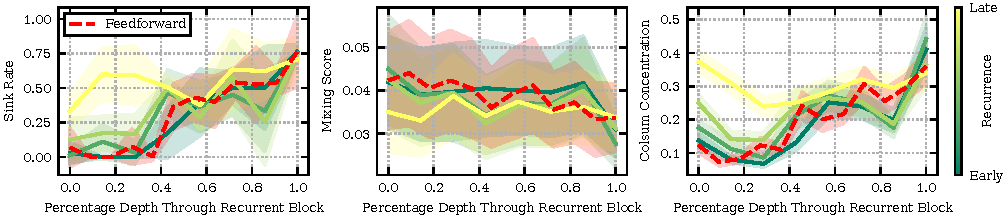
\includegraphics{figures/training/R8.pdf}
    \caption{\textbf{Stages of inference metrics for a small-scale Looped Transformer of configuration $(0,8 \otimes 4,0)$}, compared to a ``control'' feedforward Transformer with the same training configuration and depth 12.}
    \label{fig:r8}
\end{figure}

\begin{figure}[ht]
    \centering
    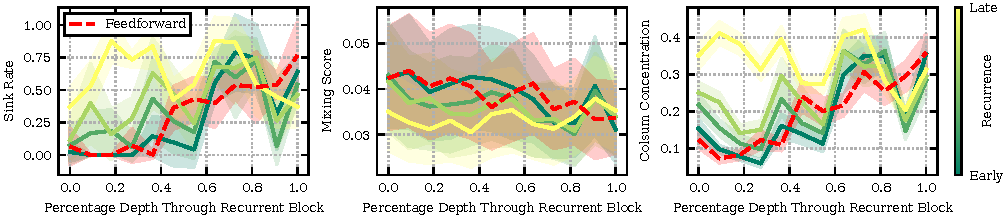
\includegraphics{figures/training/R12.pdf}
    \caption{\textbf{Stages of inference metrics for a small-scale Looped Transformer of configuration $(0,12 \otimes 4,0)$}, compared to a ``control'' feedforward Transformer with the same training configuration and depth 12.}
    \label{fig:r12}
\end{figure}

\FloatBarrier
\section{Looped Floorplan}

To illustrate the ``similar attention patterns between recurrences'' that we have discussed throughout the paper, in \Cref{fig:retrofitted_llama_floorplan} we visualize all attention patterns for the Retrofitted Llama model on the test prompt. Increasing depth in the model is aligned with increased height up the page; Prelude and coda are outlined in blue and red respectively and separate recurrences are separated by a space.

\begin{figure}[ht]
    \centering
    \includegraphics[height=0.7\textheight]{figures/floorplan/Retrofitted_Llama_8_steps.pdf}
    \caption{\textbf{Entire attention pattern floorplan for the retrofitted Llama model}, illustrating the cyclic similarity between recurrences.}
    \label{fig:retrofitted_llama_floorplan}
\end{figure}


\end{document}


% This document was modified from the file originally made available by
% Pat Langley and Andrea Danyluk for ICML-2K. This version was created
% by Iain Murray in 2018, and modified by Alexandre Bouchard in
% 2019 and 2021 and by Csaba Szepesvari, Gang Niu and Sivan Sabato in 2022.
% Modified again in 2023 and 2024 by Sivan Sabato and Jonathan Scarlett.
% Previous contributors include Dan Roy, Lise Getoor and Tobias
% Scheffer, which was slightly modified from the 2010 version by
% Thorsten Joachims & Johannes Fuernkranz, slightly modified from the
% 2009 version by Kiri Wagstaff and Sam Roweis's 2008 version, which is
% slightly modified from Prasad Tadepalli's 2007 version which is a
% lightly changed version of the previous year's version by Andrew
% Moore, which was in turn edited from those of Kristian Kersting and
% Codrina Lauth. Alex Smola contributed to the algorithmic style files.
